\pdfoutput=1
\documentclass[11pt]{amsart}
\usepackage{amsmath,amssymb,amsthm}
\usepackage[margin=1.2in]{geometry}
\usepackage{booktabs,adjustbox,graphicx,xcolor}
\usepackage{tikz}
\usepackage[colorlinks=true,linkcolor=blue,citecolor=blue,urlcolor=blue]{hyperref}
\hypersetup{pdfauthor={Bernd Johannes Wuebben},
 pdftitle={Quantitative metric wall crossing for K3 bundle moduli}}
\setlength{\emergencystretch}{2em}
\newtheorem{theorem}{Theorem}[section]
\newtheorem{proposition}[theorem]{Proposition}
\newtheorem{lemma}[theorem]{Lemma}
\newtheorem{corollary}[theorem]{Corollary}
\theoremstyle{definition}
\newtheorem{definition}[theorem]{Definition}
\newtheorem{example}[theorem]{Example}
\theoremstyle{remark}
\newtheorem{remark}[theorem]{Remark}
\newcommand{\CC}{\mathbb C}
\newcommand{\RR}{\mathbb R}
\newcommand{\ZZ}{\mathbb Z}
\newcommand{\PP}{\mathbb P}
\DeclareMathOperator{\Ext}{Ext}
\DeclareMathOperator{\Hom}{Hom}
\DeclareMathOperator{\End}{End}
\DeclareMathOperator{\tr}{tr}
\DeclareMathOperator{\rank}{rk}
\DeclareMathOperator{\Herm}{Herm}
\title{Quantitative metric wall crossing for K3 bundle moduli}
\author{Bernd Johannes Wuebben}
\subjclass[2020]{53C07 (primary); 14J28, 14D20, 53C26, 53C23 (secondary)}
\keywords{Hermitian--Einstein metric, K3 surface, quiver variety,
wall crossing, moduli metric, hyperk\"ahler quotient}
\date{November 6, 2026}


\begin{document}
\begin{abstract}
We compare harmonic $L^2$ metrics on bundle moduli over a projective
K3 surface with flat quiver quotient metrics near a polystable bundle.
Its locally free factors are slope-stable with a common reduced Hilbert
polynomial for an ample polarization, and slope-stable of a common slope
for a central Ricci-flat K\"ahler background, whose class may differ.
The multiplicative metric error tends to zero uniformly as stabilizers
change and positive degeneration scales separate arbitrarily.
The proof retains all parallel automorphisms in the finite-dimensional
reduction and computes harmonic lengths by complementary gauge minimization.
For doubled quivers admitting a representation with no nonzero proper
subrepresentation in the complex zero moment fiber, we prove pointed
Gromov--Hausdorff continuity of the complete stratified quotients as real
central parameters vary. Under this hypothesis, finite successive
rescalings of the actual moduli metric have complete limits whenever
the rescaled parameters and balanced normal base representatives converge
at each stage. We apply the method to a rank-five K3 bundle with three
spherical factors, multiplicities $(2,2,1)$, and two independent
polarization parameters. Its five realized walls have selected transverse
contractions with models $T^*\mathbb P^9$, $T^*\mathbb P^{11}$ and
$T^*\mathbb P^{17}$. We determine their contraction scales, distances to
the corresponding strata, and matching to the surrounding wall metric.
\end{abstract}
\maketitle
\enlargethispage{2pt}
\section{Introduction}\label{sec:introduction}

Near a reducible polystable bundle, deformation theory gives a finite
quotient description of the moduli germ. The harmonic $L^2$ metric
contains further information. It is obtained by solving the
Hermitian--Einstein equation and then taking harmonic representatives
of deformations. When the stabilizer changes, the finite orbit
operator develops small eigenvalues, so an inverse estimate that
treats all gauge directions together is not uniform. This distinction
is especially relevant when several stability parameters approach
different walls at different rates.

We prove a local comparison between the actual harmonic metric and
the flat quiver quotient metric that remains relative through these
degenerations. The geometric setting is a projective K3 surface with
a polystable locally free sheaf
$E_0=\bigoplus_iF_i\otimes\CC^{m_i}$.
The factors are pairwise nonisomorphic slope-stable bundles with
equal reduced Hilbert polynomial for an integral ample class.
The central analytic metric is Ricci-flat in a K\"ahler class for
which the factors are stable of a common slope; the two classes
may coincide. These hypotheses are verified directly in the
application below, including at its selected noncentral wall points.

The central harmonic norm and Serre duality identify
$V=\Ext^1(E_0,E_0)$ with a unitary doubled-quiver representation.
Its complex moment zero locus gives the convergent integrability
model. For nearby K\"ahler forms $\omega_t$, the real central
parameter is the degree difference
\[
 \zeta_i(t)=2\pi\bigl(\rank(F_i)\mu_{\omega_t}(E_0)
              -\deg_{\omega_t}F_i\bigr).
\]
Theorem~\ref{thm:harmonic-comparison} identifies full local
neighborhoods of actual HYM solutions with the corresponding
finite quotients. On each genuine smooth-stratum tangent space,
at a representative of harmonic norm $r$, it proves
\[
 f_t^*g_t^{L^2}=(1+O(|t|+r))g_{\zeta(t)}
\]
in the sense of two-sided inequalities of Hermitian forms.
The constant does not depend on stabilizer type or ratios among
positive finite orbit eigenvalues. A verified central sign symmetry
improves $r$ to $r^2$; no such cancellation is assumed otherwise.

\subsection{The analytic argument}
All parallel automorphisms are retained in the finite-dimensional
problem. On their fixed infinite-dimensional orthogonal complement,
the gauge equation has a uniformly coercive elliptic inverse.
The remaining finite moment map is the moment of a smooth closed
invariant two-form close to the flat form.

The decisive finite estimate is relative to each orthogonal
vertex projection $P$:
\[
 |\langle\rho(x)-\mu(x),P\rangle|
       \le\varepsilon\|C_xP\|^2.
\]
Here $\mu$ is the flat moment, $\rho$ the perturbed normalized
moment, and $C_x$ the infinitesimal action. The same crossing
energy appears in the positive moment increment across a spectral
cut. Working in the Hermitian centralizer of the actual compact
stabilizer, orthogonal to its infinitesimal stabilizer, makes this
crossing energy strictly positive at every nonzero boundary
correction. It cancels from the estimate. A degree argument gives
a bounded complex-orbit correction and a reverse correction
without assuming a uniform positive orbit gap.

For the metric, first minimize over the fixed complementary
gauge directions. The resulting smooth finite Hermitian form
has the flat harmonic norm as its value at the origin. Minimizing
next over the retained finite algebra gives exactly the actual
harmonic Kodaira--Spencer norm. Derivatives of the orbit correction
are complex vertical and disappear in this infimum. This yields
relative quotient estimates without bounding those derivatives.
A separate stratum implicit-function argument and a full local
inverse supply the differentiability and coverage needed in this
calculation.

These steps develop methods from the preceding stability-degeneration
papers. The spectral-cut calibration is from
\cite{Wue26a}, and its repeated-factor form is developed in
\cite{Wue26c}. Relative moduli-metric comparison by complementary
minimization is developed in \cite{Wue26b,Wue26c}.
The projection-relative moment estimate and the harmonic
coordinate argument were used for the two-factor K3 example in
\cite{Wue26d}. Here the finite correction treats arbitrary
quiver stabilizers, including loops, and its reverse direction
covers the full nearby solution space. We give the required
proofs rather than import conclusions restricted to those earlier
representations.

\subsection{Intrinsic consequences}
A comparison of tangent norms alone does not determine intrinsic
distances or a complete rescaled limit: short competing paths
could leave the chart, and an image of a fixed model ball need
not cover the corresponding actual ball. We establish both
path localization and inverse coverage.

The finite-dimensional result is also useful independently.
For any doubled quiver whose complex zero fiber contains a
module-simple representation, meaning one with no nonzero proper
subrepresentation, Theorem~\ref{thm:varying-parameters}
proves that the full stratified length quotient at every real
central parameter is a proper geodesic space.
Arbitrary converging real parameters give converging distances
for converging balanced representatives, and convergence to the
whole complete pointed quotient, including singular levels.
The proof uses connected fibers of projective face maps to
construct shrinking neighborhoods, uniform semialgebraic paths
for short joins, and a quantitative Hamiltonian slice to retain
asymptotically exact lengths along strata. Horizontal lifting
gives the opposite distance inequality.

Combining this result with the harmonic comparison gives complete
actual rescaled limits whenever $\zeta(t_n)/\delta_n^2$ converges.
At a moving wall point, the full normal Ext-quiver again has a
module-simple zero representation. Translation in its trivial
factor and another rescaling identify finer limits.
The result can be iterated through any fixed finite succession
of convergent centers and scales, under the explicit bounded
normal-parameter and base-point hypotheses of
Theorem~\ref{thm:moving-centers}. No comparability of the successive
positive scales is imposed.
We also obtain relative distances to specified conical strata,
the square-root contraction profile of compact cores, and
matching to the surrounding free wall metric in the regime
$\|\zeta\|/\lambda\to0$, where $\lambda$ is the least positive
finite orbit eigenvalue.

\subsection{The K3 application}
We realize a projective K3 surface with
$\operatorname{NS}(X)=\langle2\rangle\oplus A_2(-2)$ and an ample
class $H$. Three spherical line bundles with classes $a,b,-a-b$
have four cross-extension directions for every pair. With
multiplicities $(2,2,1)$ their direct sum has primitive Mukai
vector $(5,a+b,-5)$ of square $46$.
The resulting local moduli have complex dimension $48$.
The real polarization family $H+ta+ub$ realizes two independent
stability parameters.

The finite representation is a doubled triangle on which two
matrix groups $U(2)$ act nontrivially and interact.
Five realized wall lines meet at the central bundle and divide
the parameter plane into ten chambers.
Explicit adjoint-paired arrow matrices prove the existence of simple
representations at zero moment level for the full vector and every required wall
summand. At selected actual two-factor wall strata, the transverse
contractions have models $T^*\PP^9$, $T^*\PP^{11}$ and
$T^*\PP^{17}$, with complete product metric limits and precise
square-root contraction scales. At the wall the distance to the
two-factor stratum is $(1+O(r))\sqrt{2s}$, where $s$ is the nonzero
singular value of the rank-one square-zero transverse invariant.
Theorem~\ref{thm:k3-application} states these conclusions for the
actual harmonic metric.

The cycle, interacting matrix symmetries, and independent
parameters are essential features of this application.
There is no vertex-scalar sign acting as $-I$ on every edge,
and approaches to its intersecting walls require the singular
and iterated limit arguments. The comparison is therefore used
beyond a change of matrix size in a two-factor quotient.

\subsection{Relation to the literature and scope}
The quadratic K3 deformation model is classical in origin.
Budur--Zhang prove the required formality \cite{BZ19};
Arbarello--Sacc\`a give the equivariant analytic quadratic
identification and its quiver description
\cite[Propositions~4.4 and 6.1]{AS18}.
Their dimension-one sheaf wall-crossing theorem is not used
to identify this rank-five bundle problem.
Their later treatment of Bridgeland moduli compares nearby stability
conditions with local quiver VGIT, away from totally semistable walls
and for sufficiently close conditions with the same heart
\cite[\S6, Claim~6.1, Proposition~6.3 and Corollary~6.4]{AS25}.
This broader local comparison concerns algebraic stability and does
not supply the harmonic metric estimates studied here.
King's quotient theory \cite{King94}, Crawley-Boevey's
moment-fiber theorem \cite{CB01}, and Bellamy--Schedler's
normality and projective face maps \cite{BeSc24} supply the
algebraic geometry used here. Mayrand's full Hamiltonian slice
\cite{May22} supplies the analytic local form; we additionally
prescribe its isometric normal first jet and compare its
real quotient metric.

Buchdahl--Schumacher's analytic GIT and Weil--Petersson work
\cite{BS21,BS23,BS26} provides analytic metric antecedents.
Clarke--Tipler prove local HYM wall variation for simple sufficiently
smooth semistable bundles with abelian graded automorphism group
\cite[Proposition~1.1 and Theorem~1.2]{CT24}.
Delloque removes the abelian restriction and proves continuity of
HYM connection classes under metric variation
\cite[Theorems~4.8--4.9]{DelCont25}.
These results concern connections and graded bundles; the relative
harmonic moduli-metric estimates require the additional arguments here.
We use Delloque's later parameter-dependent local solution theory
\cite{Del25} on its integrable HYM branch for full local
classification and inverse coverage, and prove separately the
uniform estimates through the retained symmetry directions.
Namikawa--Odaka establish metric tangent-cone asymptotics under
their reduction hypotheses \cite[Setup~1, Proposition~6.10 and
Corollary~6.13]{NO26}. Their Remark~6.14 distinguishes
the metric tangent cone from the flat symplectic-slice reduction
metric, and the derivative estimate in Corollary~6.13(ii)
has an isolated-singularity hypothesis. Our conclusions concern
the stated quiver and bundle settings, with nonisolated strata
and varying real parameters; they are not a general hyperk\"ahler
equivalence theorem for arbitrary symplectic singularities.
Xu--Zhuang, with an appendix by Guenancia, prove formal conicality
and derive analytic conicality in their symplectic-singularity
setting \cite[Theorem~1.2 and Appendix~A]{XZ26}; general
hyperk\"ahler-cone existence remains their Conjecture~1.3.
These algebraic and analytic conclusions do not by themselves
give the quantitative harmonic-metric comparison proved here.

All moduli identifications and contraction maps asserted here
are local. In particular we do not identify a global metric
completion, a bubbling compactification, or an HYM evolution.
The full stratified length metric is specified explicitly;
identifying it with the completion of the regular locus alone
would be a further statement.


\section{Uniform correction in complex quiver orbits}\label{sec:balancing}

Let $Q$ be a finite quiver, allowing loops and multiple arrows.
For Hermitian spaces $W_i$ of dimensions $m_i>0$, put
\[
 V=\bigoplus_{a:i\to j}\operatorname{Hom}(W_i,W_j),\qquad
 K=\prod_iU(W_i),\qquad G=\prod_iGL(W_i).
\]
We use the Hilbert--Schmidt metric on $V$ and the ordinary trace pairing
on the real vector space $\mathfrak a=\bigoplus_i\operatorname{Herm}(W_i)$.
The action and its Hermitian infinitesimal action are
\[
 (g x)_a=g_jx_ag_i^{-1},\qquad (C_xS)_a=S_jx_a-x_aS_i.
\]
Thus the vector field generated by $iS$ is $\xi_S(x)=iC_xS$.
Our real moment map and symplectic normalization are
\begin{equation}\label{eq:moment-normalization}
 \mu_i(x)=\sum_{h(a)=i}x_ax_a^*-\sum_{t(a)=i}x_a^*x_a,
 \qquad
 d\langle\mu,S\rangle=2\omega_0(\xi_S,\cdot),
 \quad \omega_0(iC_xS,C_xS)=\|C_xS\|^2.
\end{equation}
The common scalar acts trivially. A central covector is written
$\zeta=(\zeta_i I_{W_i})$ with $\sum_i m_i\zeta_i=0$.
A \emph{subrepresentation} is a collection $D_i\subset W_i$ with
$x_aD_{t(a)}\subset D_{h(a)}$ for every arrow.
A representation is \emph{module-simple} if its only
subrepresentations are zero and itself. This condition is independent
of a stability parameter and is stronger than having only scalar
endomorphisms.

Let $\Omega$ be a smooth closed $K$-invariant two-form on the Euclidean
ball $B_R\subset V$, and let $\rho:B_R\to\mathfrak a$ be an equivariant
moment map with
\begin{equation}\label{eq:perturbed-moment}
 \rho(0)=0,\qquad
 d\langle\rho,S\rangle=2\Omega(\xi_S,\cdot),\qquad
 \|\Omega-\omega_0\|\le\varepsilon.
\end{equation}
The last norm is the Euclidean operator norm. We do not assume that
$\Omega$ is of type $(1,1)$. Its indicated bound, with $\varepsilon<1$,
implies positivity on the pairs $(iC_xS,C_xS)$ used below.
We call $x$ $\rho$-balanced at $\zeta$ if $\rho(x)=\zeta$;
flat balancing means $\mu(x)=\zeta$.

\begin{theorem}\label{thm:uniform-balancing}
There are constants $A,\varepsilon_0>0$, depending only on
$M=\sum_i m_i$, with the following properties whenever
\eqref{eq:perturbed-moment} holds and $\varepsilon<\varepsilon_0$.
\begin{enumerate}
\item If $x\in B_{R/4}$ and $\mu(x)=\zeta$ is central, there is
$S\in\mathfrak a$ with $\|S\|_{\mathrm{op}}\le A\varepsilon$ and
$\rho(e^Sx)=\zeta$.
\item If $y\in B_{R/4}$ and $\rho(y)=\zeta$ is central, there is
$T\in\mathfrak a$ with $\|T\|_{\mathrm{op}}\le A\varepsilon$ and
$\mu(e^Ty)=\zeta$.
\item In a fixed complex orbit, the $\rho$-balanced representatives in
$B_R$ at the central value $\zeta$ form at most one $K$-orbit.
The corresponding local maps between balanced compact quotients are
continuous and inverse on nested neighborhoods. These conclusions
remain valid after restriction to a $G$-invariant analytic subset of $V$.
\end{enumerate}
No bound on a positive eigenvalue of $C_x^*C_x$ is required.
\end{theorem}

The proof extends the spectral-cut and degree argument of
\cite{Wue26a,Wue26c}. The projection estimate used in
\cite{Wue26d} is the appropriate error bound: both the coercive term and
the error contain the same crossing energy. Retaining the full stabilizer
in the argument also gives the reverse assertion and continuity when
stabilizers change.

\subsection{A relative estimate for every projection}
For a tuple $P=(P_i)$ of orthogonal projections, set
\[
 q_P(x)=\|C_xP\|^2
       =\sum_{a:i\to j}\|P_jx_a-x_aP_i\|^2.
\]
\begin{lemma}\label{lem:projection-error}
Under \eqref{eq:perturbed-moment},
\[
 |\langle\rho(x)-\mu(x),P\rangle|\le\varepsilon q_P(x)
 \qquad (x\in B_R).
\]
\end{lemma}
\begin{proof}
Write each arrow in its preserving and crossing blocks for $P$, and
write $x=n+u$ for the resulting orthogonal decomposition.
The circle $\exp(itP)$ fixes $n$. On its fixed vector space both
moment components paired with $P$ have zero differential, and their
normalizations at the origin are zero. Along $n+su$ we have
$\xi_P=s\,iC_uP$ and $\|C_uP\|=\|u\|$. Orthogonality keeps this segment
in $B_R$. The moment identities give
\[
 \langle\rho(x)-\mu(x),P\rangle
 =2\int_0^1s(\Omega-\omega_0)_{n+su}(iC_uP,u)\,ds.
\]
Its absolute value is at most $\varepsilon\|u\|^2=\varepsilon q_P(x)$.
\end{proof}

\subsection{The stabilizer and a strict spectral cut}
Fix $x$, let $H=K_x$, and define
\[
 \mathfrak h=\{S\in\mathfrak a:C_xS=0\},\qquad
 \mathfrak c=\{S\in\mathfrak a:Sh=hS\text{ for all }h\in H\},
 \qquad \mathfrak p=\mathfrak c\cap\mathfrak h^\perp.
\]
The commutation condition is understood vertexwise.
If $S\in\mathfrak p$, then $e^Sx\in V^H$. Any normalized equivariant
moment map takes its values on $V^H\cap B_R$ in $\mathfrak p$:
equivariance puts the value in $\mathfrak c$, and the vanishing
generating fields of $\mathfrak h$ show that its pairing with
$\mathfrak h$ is constant, hence zero, on this connected fixed ball.
In particular a central target attained at $x$ belongs to $\mathfrak p$.
Order the union of the spectra of all vertex matrices $S_i$,
including multiplicities. Adjacent eigenvalues below refer to this
single ordered list.

\begin{lemma}\label{lem:strict-cut}
If $S\in\mathfrak p$ and $\|S\|_{\mathrm{op}}=a>0$, there is a
global adjacent eigenvalue gap of size at least $a/(M-1)$.
For the vertexwise spectral projection $P$ above any strict global gap,
$q_P(x)>0$.
\end{lemma}
\begin{proof}
The identity tuple belongs to $\mathfrak h$, so $\operatorname{tr}S=0$.
The oscillation of its $M$ eigenvalues is at least $a$, proving the
gap estimate. A spectral projection $P$ commutes with $H$. If
$q_P(x)=0$, it also belongs to $\mathfrak h$. Since $I-P\in\mathfrak h$,
orthogonality gives
$\operatorname{tr}(SP)=\operatorname{tr}(S(I-P))=0$.
The mean eigenvalues above and below a strict gap cannot both vanish.
\end{proof}
For $M=1$ the action is trivial and all normalized moments vanish.
The following proof therefore assumes $M\ge2$.

\subsection{The forward and reverse degree arguments}
\begin{proof}[Proof of Theorem~\ref{thm:uniform-balancing}]
When $\varepsilon=0$, the moment identities and the common
normalization give $\rho=\mu$, so take zero correction. Assume
$\varepsilon>0$. We may take
\[
 A=2M,\qquad \varepsilon_0=\frac{\log2}{16A},\qquad a=A\varepsilon.
\]
If $\mathfrak p=0$, both moments at the starting point vanish and no
correction is needed. Otherwise consider, on the operator-norm ball of
radius $a$ in $\mathfrak p$,
\[
 F_s(S)=\mu(e^Sx)-\zeta+s(\rho-\mu)(e^Sx),\qquad 0\le s\le1.
\]
This homotopy takes values in the same fixed space $\mathfrak p$.
All its arguments have norm at most $e^{2a}\|x\|<R/2$.

At a boundary point diagonalize $S$ vertexwise and choose $P$ above
a gap $\delta\ge a/(M-1)$. An arrow entry with eigenvalue difference
$d$ has squared norm multiplied by $e^{2d}$. For an entry crossing
into $P$ the contribution to the paired moment increment is
$(e^{2d}-1)w$, with $d\ge\delta$; for one crossing out it is
$(1-e^{2d})w$, with $d\le-\delta$. Therefore
\begin{align}
 \langle\mu(e^Sx)-\mu(x),P\rangle
 &\ge(1-e^{-2\delta})q_P(x)
 \ge 2e^{-4a}\frac{a}{M-1}q_P(x), \label{eq:cut-lower}\\
 |\langle(\rho-\mu)(e^Sx),P\rangle|
 &\le\varepsilon e^{4a}q_P(x).                    \label{eq:cut-error}
\end{align}
Here $\delta\le2a$, and $P$ commutes with $S$.
Our constants make the first coefficient strictly larger than the
second. Lemma~\ref{lem:strict-cut} makes the crossing energy positive.
Thus $F_s$ has no boundary zero; no continuous choice of $P$ is needed.

The only zero of $F_0$ is $S=0$. Indeed
\[
 \frac{d}{dt}\langle\mu(e^{tS}x),S\rangle
   =2\|C_{e^{tS}x}S\|^2
\]
is strictly positive for $S\in\mathfrak p\setminus\{0\}$:
$C_{e^{tS}x}S=e^{tS}C_xS$, and $C_xS=0$ would imply
$S\in\mathfrak h\cap\mathfrak h^\perp$.
Moreover $DF_0(0)$ has positive quadratic form $2\|C_xS\|^2$ on
$\mathfrak p$, so its local degree is $+1$.
Brouwer degree gives a zero of $F_1$. This uses invertibility at each
fixed $x$, not a uniform lower eigenvalue estimate.

For the reverse assertion set $E=\rho-\mu$, define $\mathfrak p$
using $H=K_y$, and use
\[
 G_s(S)=\mu(e^Sy)-\mu(y)-sE(y).
\]
All terms again lie in $\mathfrak p$. Its initial zero is unique and
nondegenerate by the preceding calculation, which does not require
$\mu(y)$ to be central. On the boundary \eqref{eq:cut-lower} dominates
$|\langle E(y),P\rangle|\le\varepsilon q_P(y)$.
A zero at $s=1$ satisfies $\mu(e^Sy)=\rho(y)=\zeta$.
This proves existence of a flat balanced representative without an
independent polystability assumption.

For uniqueness suppose $y,gy\in B_R$ are $\rho$-balanced at the same
central value. Write $g=ke^T$. Equivariance and centrality reduce to
$y,e^Ty$. In an eigenbasis of $T$, the squared norm of $e^{sT}y$
is a sum of nonnegative exponentials, hence convex on $[0,1]$.
The entire path therefore stays in $B_R$, and
\[
 \frac{d}{ds}\langle\rho(e^{sT}y),T\rangle
 =2\Omega(iC_{e^{sT}y}T,C_{e^{sT}y}T)
 \ge2(1-\varepsilon)\|C_{e^{sT}y}T\|^2.
\]
Its endpoint values agree, so $C_yT=0$, and $gy=ky$.

Both corrections remain in any invariant analytic subset.
Uniqueness makes the compact-orbit maps independent of all choices.
For continuity choose convergent representatives and bounded correction
matrices. Every convergent subsequence of those matrices supplies a
balanced limit in the same complex orbit; uniqueness identifies its
compact orbit. The limiting matrix need not lie in the limiting
$\mathfrak p$. Compactness in the full fixed Hermitian algebra suffices.
The same proof gives parameter continuity for smooth families with a
common bound.

For explicit domains write
$\mathcal A_s=(Z\cap\mu^{-1}(\zeta)\cap B_s)/K$ and
$\mathcal B_s=(Z\cap\rho^{-1}(\zeta)\cap B_s)/K$.
The forward and reverse maps send radius $R/4$ into radius $R/2$
and are inverse wherever both are defined. In particular the forward
map identifies $\mathcal A_{R/8}$ with the open subset
$g^{-1}(\mathcal A_{R/8})$ of $\mathcal B_{R/4}$, where $g$ denotes
the reverse map; its image contains $\mathcal B_{R/16}$.
This proves the local statement with the required slack in radii.
\end{proof}

\begin{corollary}\label{cor:balancing-rate}
For a jointly smooth family satisfying
$\|\Omega_t-\omega_0\|_{B_{2r}}\le C(|t|+r^\alpha)$,
the correction on a fixed inner subball has norm
$O(|t|+r^\alpha)$, uniformly in stabilizer type and ratios of
nonzero arrow sizes. Smooth normalization gives $\alpha=1$.
The value $\alpha=2$ follows if the first spatial derivative vanishes,
for example under a verified inversion symmetry.
\end{corollary}
\begin{proof}
Apply Theorem~\ref{thm:uniform-balancing} on $B_{2r}$.
Taylor's theorem gives the two stated rates under their respective
derivative hypotheses.
\end{proof}
The theorem alone asserts neither differentiability across strata nor
a metric comparison. Both require identifying genuine tangent vectors
and removing complex gauge directions; we do this next.


\section{Harmonic coordinates and the metric on K3 bundle moduli}
\label{sec:harmonic}

Let $X$ be a projective K3 surface and $H$ an integral ample class.
Let $F_1,\ldots,F_l$ be pairwise nonisomorphic locally free
$H$-slope-stable sheaves with the same reduced $H$-Hilbert polynomial.
Fix positive multiplicities $m_i$ and put
\[
 E_0=\bigoplus_i F_i\otimes W_i,\qquad W_i=\CC^{m_i}.
\]
For the central analytic background choose a real K\"ahler class
$\omega_*$ for which the same $F_i$ are slope-stable of a common slope,
and use its Ricci-flat K\"ahler metric. One may take $\omega_*=H$.
These are separate hypotheses: $H$ supplies algebraic formality,
whereas $\omega_*$ supplies the Hermitian--Einstein background.
Choose its direct-sum Hermitian--Einstein metric $h_0$ on $E_0$.
Fix the determinant, and let $\omega_t$ be a smooth finite-dimensional
family of K\"ahler forms with $\omega_0=\omega_*$.

Give $V=\Ext^1(E_0,E_0)$ its central harmonic Hermitian norm.
Serre duality identifies it unitarily with a doubled-quiver
representation for $K=\prod_iU(W_i)$; self-extensions give paired
loops, as proved below. Let $\mu_{\CC},\mu$ be its complex and real
moments with the normalization of \eqref{eq:moment-normalization},
and put $Z=\mu_{\CC}^{-1}(0)$.
For $r_i=\rank F_i$ and $N=\sum_i r_im_i$, define
\begin{equation}\label{eq:geometric-parameter}
 \zeta_i(t)=2\pi\bigl(r_i\mu_{\omega_t}(E_0)
                  -\deg_{\omega_t}F_i\bigr),
 \qquad \sum_i m_i\zeta_i(t)=0.
\end{equation}
Degrees mean $\int_Xc_1(F_i)\wedge\omega_t$ and slope is degree
divided by rank. In particular \eqref{eq:geometric-parameter}
has no volume denominator.
This sign agrees with the incoming-minus-outgoing convention:
a subbundle of smaller slope has positive total $\zeta$-weight.

At a balanced quiver point, decompose the representation into
pairwise nonisomorphic stable summands. Its \emph{representation type}
is the unordered list of their dimension vectors and multiplicities.
Stability here means strictly positive $\zeta$-weight on every
nonzero proper subrepresentation; Proposition~\ref{prop:real-polystability}
justifies this decomposition. The connected strata of a fixed type
are the orbit-type strata for the compact group action. We use
these strata, including singular types, throughout the metric statements.

\begin{theorem}\label{thm:harmonic-comparison}
Under these hypotheses there are common nested neighborhoods in
which the finite quotients
\[
 M_{\zeta(t)}=(Z\cap\mu^{-1}(\zeta(t)))/K
\]
identify with open neighborhoods in the actual fixed-determinant
Hermitian--Yang--Mills bundle moduli. Every sufficiently small actual
solution for sufficiently small $t$ is covered. The maps $f_t$ are
homeomorphisms, smooth on representation-type strata, and preserve
their complex structures. On genuine stratum tangents at a finite
representative $x$, with $r=\|x\|$,
\begin{equation}\label{eq:harmonic-comparison}
 (1-C(|t|+r))g_{\zeta(t)}
 \le f_t^*g_t^{L^2}
 \le(1+C(|t|+r))g_{\zeta(t)}.
\end{equation}
The constants are independent of stabilizer type and of ratios of
positive eigenvalues of the finite orbit operator.

If a central unitary automorphism acts as $-I$ on all of $V$, the
spatial error in \eqref{eq:harmonic-comparison} improves to $Cr^2$.
At the central value the construction identifies the full reduced
analytic quotient germ, including its singular locus.
\end{theorem}

Here a neighborhood of actual solutions means solutions represented
by small deformations of the fixed smooth bundle and central
Dolbeault operator, uniformly in $t$. The central holomorphic bundle
itself need not remain polystable when $t\ne0$.
The proof combines a fixed elliptic inverse with
Theorem~\ref{thm:uniform-balancing}. The elliptic inverse removes the
whole parallel algebra; no potentially small finite symmetry is
included in that inverse. The complementary minimization method
of \cite{Wue26b,Wue26c,Wue26d} then yields the metric estimate.

\subsection{Unitary quiver coordinates}
Write $d=\bar\partial_0$ on $\End E_0$ and identify $V$ with its
harmonic degree-one forms. Fix a parallel holomorphic two-form
$\Omega_X$ with normalization compatible with the harmonic norm.
In unitary coframes and factor frames define
\[
 J_{ij}(A_1\bar\theta^1+A_2\bar\theta^2)
       =-A_2^*\bar\theta^1+A_1^*\bar\theta^2.
\]
This is frame-independent, antiunitary, and maps the $(i,j)$ factor
space to the $(j,i)$ space, with $J_{ji}J_{ij}=-I$.
Choose the orientation of the Serre pairing
$Q(\alpha,\gamma)=\int_X\Omega_X\wedge\tr(\alpha\wedge\gamma)$
so that
\[
 Q(\alpha,J\beta)=\langle\alpha,\beta\rangle_{L^2}.
\]
Pointwise this is the identity
$\tr(A_1B_1^*+A_2B_2^*)$.
If $\beta$ is harmonic, its orthogonality to exact forms and Stokes'
formula show $dJ\beta=0$. Apply the opposite pairing, $J^2=-I$ and
Stokes' formula to show that $J\beta$ is orthogonal to exact forms
as well. Thus $J$ preserves harmonicity; flat factor connections
are not assumed.

Paired orthonormal bases identify off-diagonal extension spaces
with opposite arrows. Each diagonal $\Ext^1(F_i,F_i)$ is
quaternionic; choose pairs $\alpha,J\alpha$, each giving loop
coefficients $A,B\in\End W_i$. The quadratic Yoneda contribution
of this pair is $[A,B]$. In the Serre-dual target paired with the
parallel algebra by ordinary multiplicity trace, the total quadratic
obstruction is exactly $\mu_{\CC}$.
If $\eta_X$ generates $H^{0,2}(\mathcal O_X)$ with
$\int_X\Omega_X\wedge\eta_X=1$, its literal harmonic block
representative is instead
\begin{equation}\label{eq:rank-dual}
 \bigoplus_i r_i^{-1} I_{F_i}\otimes\mu_{\CC,i}\,\eta_X.
\end{equation}
The factors $r_i^{-1}$ compensate for tracing $I_{F_i}$.
The ordinary finite dual and these harmonic block coefficients
must not be interchanged.

\subsection{Convergent quadratic integrability coordinates}
The harmonic Kuranishi embedding on a full ball is the convergent
solution of
\begin{equation}\label{eq:kuranishi-embedding}
 \Phi(b)=b-d^*G_2(\Phi(b)\wedge\Phi(b)),\qquad D\Phi(0)=\iota.
\end{equation}
Here $G_2$ is the Green operator for the degree-two Dolbeault
Laplacian at the central bundle. The elliptic contraction construction is holomorphic, and its
Green operators commute with the parallel multiplicity action.
Its integrability locus has a reduced analytic germ $S\subset V$.
Reduced analytic semiuniversality is provided by
\cite[\S5 and Remark~4]{BS21}.

The bundle $E_0$ is $H$-Gieseker polystable. Budur--Zhang
\cite[Theorem~1.2]{BZ19} gives formality of its derived
endomorphism algebra. The equivariant analytic result of
Arbarello--Sacc\`a \cite[Proposition~4.4]{AS18}, with the quiver
identification in their Proposition~6.1, identifies the reduced
Quot slice with the quadratic germ $Z$, tangent to the identity.
This is a fixed-bundle germ result. We do not invoke their
dimension-one sheaf wall-crossing theorem for vector bundles.

We record the analytic comparison with the harmonic family,
because formality alone would not supply controlled harmonic
coordinates. Twist the harmonic family by a sufficiently large
multiple of $H$. Analytic base change makes its spaces of sections
a vector bundle with surjective evaluation map
\cite[Corollaries~1.4--1.5 and Theorem~3.1]{Gro61a}.
Average a holomorphic frame over $K$; it remains a frame near the
origin and makes the evaluation equivariant.
The analytic Quot construction \cite[Theorem~1.1]{Gro61b} gives a
classifying map. An equivariant complement to the stabilizer in
the ambient general linear algebra, followed by Luna's slice
\cite{Lun73}, gives a $K$-equivariant germ map
$h:S\to Z_{\rm Quot}$ with identity Kodaira--Spencer derivative.

The reduced tangent space of $Z$ is all of $V$: every subspace
supported on a single arrow, including a single loop with its
paired loop zero, lies in $Z$, and these subspaces span $V$.
First apply reduced semiuniversality to the Quot family to obtain
a reverse map $g:Z_{\rm Quot}\to S$. Its Kodaira--Spencer derivative,
followed by harmonic inclusion, is the identity on $V$.
Thus the reduced tangent of $S$ is also $V$.
This argument does not assert that an arbitrary matrix-valued
harmonic self-extension squares to zero as a differential form.

Both compositions have invertible tangent maps and are analytic
germ isomorphisms. For completeness, lift a self-map with invertible
tangent map to an ambient local biholomorphism in a minimal embedding.
Its pullback on the germ's local ring is surjective.
A surjective endomorphism of a Noetherian ring is injective:
the ascending kernels of its powers stabilize, and surjectivity
then forces its first kernel to vanish. This proves the assertion,
and hence $h$ is an isomorphism.

Extend the resulting coordinate functions to an ambient holomorphic
map and average over $K$. We obtain an equivariant local
biholomorphism $F$ satisfying
\begin{equation}\label{eq:ambient-coordinates}
 \begin{aligned}
 F(x)&=x+O(\|x\|^2),& DF(x)&=I+O(\|x\|),\\
 a(x)&=\Phi(F(x)),& D_x&=d+[a(x),\cdot],\qquad J_x=Da(x).
 \end{aligned}
\end{equation}
Its integrable locus is exactly $Z$ on suitably small representatives.
Compact equivariance complexifies locally, and for every parallel
complex endomorphism $\xi$ gives the exact identity
\begin{equation}\label{eq:exact-gauge-derivative}
 D_x\xi=-J_xC_x\xi.
\end{equation}
For a genuine tangent $v$ to an integrable stratum,
$D_x(J_xv)=0$, by differentiation of integrability.

If formality or the convergent analytic comparison is unavailable,
one must retain the full higher-order Kuranishi obstruction.
Neither a quadratic tangent obstruction nor a formal equivalence
alone justifies the homogeneous quotient and its rescalings.

\subsection{The fixed complementary gauge equation}
Use $h_0$ and its density $dV_0$ to define the Hermitian moment
\[
 \mathcal M_t=i(F^0\wedge\omega_t)/dV_0,
\]
where $F^0$ is the trace-free curvature of the unitary connection
determined by a Dolbeault operator. Let $Q_0$ be the fixed
$L^2$-orthogonal complement of the entire parallel trace-free
Hermitian algebra. The derivative in $s$ at the origin of
\[
 (t,x,s)\longmapsto
 Q_0\mathcal M_t\bigl(e^s\cdot(\bar\partial_0+a(x))\bigr)
\]
is a fixed nonzero multiple of the covariant Laplacian on $Q_0$.
All of its kernel has been removed. On fixed Sobolev spaces
$W^{k+2,2}\to W^{k,2}$, $k>2$, the implicit-function theorem gives
a unique small smooth $\sigma(t,x)\in Q_0$.
Harmonicity and the K\"ahler identities kill its first $x$ derivative
at $(0,0)$. Elliptic regularity gives, for every fixed $j$,
\begin{equation}\label{eq:complementary-correction}
 \|\sigma(t,x)\|_{C^j}\le C_j(|t|+\|x\|^2).
\end{equation}
Uniqueness gives $K$-equivariance.
Only this fixed elliptic complement is inverted.

Put $\Psi_t(x)=e^{\sigma(t,x)}\cdot(\bar\partial_0+a(x))$.
For $S\in\bigoplus_i\Herm W_i$ use the trace-free lift
\[
 \widehat S=\bigoplus_i I_{F_i}\otimes(S_i-c(S)I_{W_i}),
 \qquad c(S)=\frac{\sum_i r_i\tr S_i}{N}.
\]
Define the finite moment $m_t$ in the ordinary multiplicity dual by
\[
 \sum_i\tr(m_{t,i}(x)S_i)
   =\int_X\tr(\mathcal M_t(\Psi_t(x))\widehat S)\,dV_0.
\]
Its vanishing is equivalent to vanishing of the remaining parallel
component. This is not the rank-and-volume-weighted coefficient
of the orthogonal parallel projection. The determinant character
on $G$ is $\prod_i(\det g_i)^{r_i}$; using the ineffective common
scalar and this lift avoids an incorrect unweighted determinant
normalization.

Pullback of the affine unitary-connection symplectic form gives
a smooth closed invariant two-form $\Omega_t$ on the full ball.
In Dolbeault tangent coordinates our affine form is
$\operatorname{Im}\langle\alpha,\beta\rangle_{L^2(\omega_t)}$,
where the Hermitian pairing is linear in its first argument.
Thus the $+iF^0$ convention gives the quadratic moment $+\mu$
and $\Omega_{0,0}(iC_xS,C_xS)=\|C_xS\|^2$.
The exact moment identity is
$d\langle m_t,S\rangle=2\Omega_t(\xi_S,\cdot)$.
Since $D\Psi_0(0)$ is harmonic inclusion,
\begin{equation}\label{eq:ambient-form-estimate}
 \Omega_{0,0}=\omega_0,\qquad
 \|\Omega_{t,x}-\omega_0\|\le C(|t|+\|x\|).
\end{equation}
This proves positivity on the ordered orbit pairs used in
Section~\ref{sec:balancing}; compatibility with the original
complex structure is not needed.

At $x=0$, equivariance makes $\sigma(t,0)$ lie in
$\bigoplus_i\End F_i\otimes I_{W_i}$. It need not be scalar on $F_i$,
but preserves the factor decomposition. Chern--Weil therefore gives
\[
 \langle m_t(0),S\rangle
 =2\pi\sum_i\deg_{\omega_t}F_i\,
       \tr(S_i-c(S)I_{W_i})
 =-\sum_i\zeta_i(t)\tr S_i.
\]
The normalized moment $\rho_t=m_t-m_t(0)$ has target
$\rho_t=\zeta(t)$. Its complement has already been solved, so this
is exactly the remaining projective HYM equation.
The sign can also be checked on a single extension arrow
$A:F_i\to F_j$. Its moment is negative at $i$ and positive at $j$.
The corresponding extension $0\to F_j\to E\to F_i\to0$
can be stable only when $\mu(F_j)<\mu(E)$, precisely the sign
$\zeta_j>0$ in \eqref{eq:geometric-parameter}.
The scalar determinant equation is solved separately.
On a K3 surface $H^1(\mathcal O_X)=0$, so fixed determinant removes
no scalar degree-one deformation; its Hermitian metric does not
alter the endomorphism-valued norm.

Theorem~\ref{thm:uniform-balancing}, applied on a ball proportional
to $\|x\|$, now gives forward and reverse corrections of norm
$O(|t|+\|x\|)$ in the full multiplicity group.
They remain in $Z$ and work for every stabilizer.

\subsection{Complementary minimization and harmonic lengths}
Transport the metric to the uncorrected holomorphic family by
$H_{t,x}=h_0e^{2\sigma(t,x)}$.
Let $\mathfrak g_0$ be the full parallel complex trace-free algebra
and $Q$ its fixed $L^2$-orthogonal complement in zero-forms.
At the central point,
$\|\eta\|_{W^{1,2}}\le C\|d\eta\|_{L^2}$ on $Q$.
Smallness of $a(x)$ in $C^0$ preserves this bound with $D_x$;
nearby Hermitian and K\"ahler norms are uniformly equivalent.
Define by polarization
\begin{equation}\label{eq:complementary-minimum}
 \mathcal B_{t,x}(v,v)
 =\inf_{\eta\in QW^{1,2}}
        \|J_xv-D_x\eta\|_{H_{t,x},\omega_t}^2.
\end{equation}
The minimizing normal operator has coercive bilinear form
$\langle D_x\eta,D_x\nu\rangle$ on a fixed Hilbert space.
Its bounded inverse varies smoothly. Thus $\mathcal B$ is smooth,
positive near the origin and equivariant, and harmonic orthogonality
gives $\mathcal B_{0,0}=g_{\rm flat}$. Consequently
\begin{equation}\label{eq:complementary-metric}
 (1-C(|t|+\|x\|))g_{\rm flat}
 \le\mathcal B_{t,x}
 \le(1+C(|t|+\|x\|))g_{\rm flat}.
\end{equation}

Split every gauge zero-form into its parallel and complementary
parts. Equation~\eqref{eq:exact-gauge-derivative} gives
\begin{equation}\label{eq:full-gauge-minimum}
 \inf_\gamma\|J_xv-D_x\gamma\|^2
 =\inf_{\xi\in\mathfrak g_0}
       \mathcal B_{t,x}(v-C_x\xi,v-C_x\xi).
\end{equation}
At an integrable HYM point and a genuine stratum tangent,
Hodge theory identifies the left side with the harmonic
Kodaira--Spencer norm. A changing gauge adds an exact $D_x$ term
and conjugates isometrically, so its derivative disappears from
this minimum. We do not identify arbitrary Zariski tangent vectors
at a singular coarse point with metric tangent vectors.

For a tangent lift at a flat balanced point, differentiating the
real moment equation gives orthogonality to Hermitian orbit
directions. At a central value, Hermitian and unitary orbit
directions are orthogonal. Hence the usual quotient norm equals
\[
 \inf_{\xi\in\mathfrak g}\|v-C_x\xi\|^2
\]
on these balanced stratum tangents.
If the correction is locally $y=g(x)x$, its derivative is
$g(x)v$ plus a complex vertical vector, which disappears under
this infimum. At the point we may take the bounded $g=e^S$
from Theorem~\ref{thm:uniform-balancing}. Its squared ambient
norm distortion is between $e^{-4\|S\|_{\rm op}}$ and
$e^{4\|S\|_{\rm op}}$, and it maps complex orbit directions onto
complex orbit directions. Equations~\eqref{eq:complementary-metric}
and \eqref{eq:full-gauge-minimum} therefore yield
\eqref{eq:harmonic-comparison} without estimating $Dg$ or
inverting a small orbit eigenvalue.

A smooth local correction on each stratum exists as follows.
Fix a balanced $x_0$ with compact stabilizer $H$ and bounded
correction $S_0\in\mathfrak p_H$, and set $y_0=e^{S_0}x_0$.
Polar convexity gives $G_{x_0}=H^\CC$.
Because $S_0$ commutes with $H^\CC$, we have
$G_{y_0}=H^\CC$ and $K_{y_0}=H$.
On $V^H$ the map
\[
 (T,u)\longmapsto\rho_t(e^Te^{S_0}u)-\zeta(t),
 \qquad T\in\mathfrak p_H,
\]
takes values in that fixed space. Its derivative in $T$ at
$(0,x_0)$ has quadratic form
$2\Omega_{t,y_0}(iC_{y_0}T,C_{y_0}T)>0$ for $T\ne0$.
It is invertible at this point. The finite implicit-function
theorem gives a smooth local choice, and a compact orbit-type
slice and uniqueness identify the choices on overlaps.
At $x_0$ it is the bounded correction already used.
The local domains may shrink as orbit eigenvalues vanish; the
pointwise relative constant does not. The same argument applies
to the inverse. The holomorphic harmonic/Quot map and correction
within complex orbits preserve the complex quotient structures
on these strata.

\subsection{Full coverage and the analytic quotient}
The slice must cover all nearby actual solutions, not merely
construct a family of examples. We use the integrable HYM branch
of Delloque \cite{Del25}: the HYM subsolution condition is automatic
in \S3.2; Proposition~4.3 gives harmonic local classification,
Proposition~4.5 the complementary equation, Corollary~5.2 the
nearby morphism identification, and Proposition~5.6 the
common-parameter inverse. Lemma~7.3 and Theorem~7.4 give an
open-image homeomorphism for the integrable solution quotient.
The central solution is integrable; stable factors are simple
with vanishing cross-Hom, as required.
The possible nonintegrable failure of openness is not used.

To match its gauge normalization with ours, let $e^s$ be the
positive part of a small gauge from a harmonic representative
to an actual solution. Change the harmonic base by $e^h$ with
$h$ parallel. The new positive logarithm is
\[
 L(s,h)=\tfrac12\log(e^{-h}e^{2s}e^{-h}).
\]
Its parallel projection has derivative $-I$ in $h$ at zero.
The finite implicit-function theorem makes $L$ complementary
on a common parameter neighborhood. After unitary gauge,
uniqueness identifies it with $\sigma(t,x')$.
The reverse finite correction then provides a flat balanced
representative. Conversely every integrable zero of the corrected
moment is projectively HYM, and the determinant equation makes
it HYM. High-Sobolev classification and elliptic regularity give
the asserted smooth topology and full inverse coverage.
Nested neighborhoods are essential; no same-radius truncation
or identification of a whole noncompact quotient with a small
actual chart is claimed.

At the central value, the equivariant harmonic-to-Quot analytic
germ isomorphism descends through the analytic good quotient.
Invariant holomorphic functions pull back to invariant holomorphic
functions, so the universal property gives an isomorphism of
full reduced complex-space germs, not just their strata.
The forward and reverse moment correction identify the closed
orbits with actual HYM classes. This also applies with $H$ and
$\omega_*$ distinct under the stated hypotheses.
At a generic nonzero level the entire source chart is stable
and smooth, so the stratumwise holomorphic identification already
identifies its full complex structure.
No global comparison of nearby slope and Gieseker stability
is assumed: the latter is used at the central point for its
analytic germ.

Finally suppose a central unitary acts by $-I$ on $V$.
All ambient constructions are equivariant. The map $F$ is odd
and the coefficient matrices of $\Omega_t$ and $\mathcal B_{t,x}$
are even in $x$. Taylor expansion improves both errors to
$O(|t|+\|x\|^2)$; the same balancing and minimization proofs give
the improved rate. This completes the proof of
Theorem~\ref{thm:harmonic-comparison}.


\section{Metric slices and real stability}\label{sec:slices}

We first identify the complex quotients at arbitrary real parameters.
This also gives a properness estimate for the whole family, which will
be needed for intrinsic metric convergence. We then prove a quantitative
slice theorem at an arbitrary singular point.

\subsection{Balancing at arbitrary real parameters}
For a quiver representation $x$ of dimension $m$, a collection
$D=(D_i\subset W_i)$ is a subrepresentation if
$x_aD_{t(a)}\subset D_{h(a)}$ for every arrow.
Let $\eta\in\mathbb R^{Q_0}$ satisfy $\eta\cdot m=0$.
We call $x$ $\eta$-semistable if $\eta\cdot\dim D\ge0$ for every
subrepresentation, and $\eta$-stable if the inequality is strict for
every nonzero proper subrepresentation. It is $\eta$-polystable if
it is a direct sum of $\eta$-stable representations, each of total
$\eta$-weight zero. These definitions use arbitrary real $\eta$.

\begin{proposition}\label{prop:real-polystability}
An orbit $Gx$ meets $\mu^{-1}(\eta)$ if and only if $x$ is
$\eta$-polystable. The intersection is one $K$-orbit.
For a balanced point, $G_x$ is the complexification of $K_x$.
A stable representation has only scalar endomorphisms.
\end{proposition}
\begin{proof}
For stable $x$, consider the left $K$-invariant function
\[
 \mathcal F(g)=\|gx\|^2-2\sum_i\eta_i\log|\det g_i|.
\]
Multiplying by a common positive scalar does not change it.
Polar decomposition therefore reduces minimization to
\[
 F(S)=\|e^Sx\|^2-2\langle\eta,S\rangle,\qquad
 S\in\mathfrak a,\quad \operatorname{tr}S=0.
\]
This function is proper. Indeed, let $\|S_n\|=r_n\to\infty$ and
pass to a subsequence with $S_n/r_n\to T$, $\|T\|=1$.
Diagonalize vertexwise and pass to convergent unitary eigenbases and
normalized eigenvalues. If a nonzero coefficient of $x$ in the limiting
bases goes from a $T$-eigenvalue $\tau$ to a larger $\tau'$, its
contribution to $\|e^{S_n}x\|^2$ grows at least exponentially in $r_n$,
whereas the trace term is linear.

Otherwise every cumulative lower eigenspace of $T$ is invariant.
For its distinct global eigenvalues $\tau_1<\cdots<\tau_l$, let
$D_j=W_{\le\tau_j}$ and let $P_j$ be the corresponding projection.
There are at least two distinct eigenvalues, since $T$ is nonzero
and trace-free. Thus
\[
 T=\tau_l I-\sum_{j<l}(\tau_{j+1}-\tau_j)P_j,\qquad
 \langle\eta,T\rangle
 =-\sum_{j<l}(\tau_{j+1}-\tau_j)\eta\cdot\dim D_j<0.
\]
It follows that $F(S_n)\ge-2r_n\langle\eta,S_n/r_n\rangle\to\infty$.
These subsequence alternatives prove properness. A minimum exists,
and varying $\mathcal F$ by $g\mapsto e^{tA}g$ gives
$2\langle\mu(gx)-\eta,A\rangle=0$ for every Hermitian $A$.
The scalar equation vanishes identically, so $\mu(gx)=\eta$.

For a balanced representation and an invariant $D$, compression of the
moment equations by the orthogonal projection $P_D$ gives
\begin{equation}\label{eq:subrepresentation-trace}
 \eta\cdot\dim D
 =\sum_a\|P_{D_{h(a)}}x_a(1-P_{D_{t(a)}})\|^2\ge0.
\end{equation}
Equality means that $D$ is reducing. Split orthogonally whenever
equality occurs for a proper nonzero $D$ and induct on total dimension.
This gives stable summands of zero total weight. Conversely balance
each stable summand by the preceding minimization and take their
orthogonal direct sum.

Uniqueness follows from polar decomposition and convexity as in
Theorem~\ref{thm:uniform-balancing}: for balanced $x,e^Sx$ the function
$\|e^{tS}x\|^2-2t\langle\eta,S\rangle$ has zero endpoint derivatives
and second derivative $4\|C_{e^{tS}x}S\|^2$, so $e^Sx=x$.
If $g$ stabilizes $x$, its compact and positive polar factors
therefore both stabilize $x$, proving $G_x=(K_x)^{\mathbb C}$.

Finally, a nonzero singular endomorphism of a stable representation
would have nonzero proper kernel and image, both of positive weight,
while their weights add to zero. Every nonzero endomorphism is
therefore invertible. Subtracting an eigenvalue proves it scalar.
\end{proof}

The proposition is the polystable form of the real Kempf--Ness
criterion. Its direct proof avoids any genericity restriction.
In particular, a balanced orbit with a positive-dimensional stabilizer
is not incorrectly declared stable.

\subsection{Invariant properness and fixed faces}
From now on $V$ is a doubled-quiver representation, with
$Z=\mu_{\mathbb C}^{-1}(0)$ given its reduced structure.
Choose positive-degree homogeneous generators $f_1,\ldots,f_q$ of
$\mathbb C[Z]^G$, of degrees $d_j$, and set
$a(x)=\max_j|f_j(x)|^{1/d_j}$; set $a=0$ if there are no generators.
Finite generation is the standard reductive invariant-theory theorem
\cite[\S1.6]{KP96}.

\begin{lemma}\label{lem:invariant-properness}
There is a constant $C$ such that
\begin{equation}\label{eq:invariant-properness}
 \|x\|\le C\bigl(\|\mu(x)\|^{1/2}+a(x)\bigr),\qquad x\in Z.
\end{equation}
Consequently the family of balanced compact quotients maps properly
to the product of the central real parameter space and $Z/\!/G$.
Representatives in the affine fiber over the origin satisfy
$\|x\|\le C\sqrt{\|\eta\|}$.
\end{lemma}
\begin{proof}
The right-hand parenthesis is strictly positive on the unit sphere
in $Z$. A zero there would be balanced at zero and have all invariant
coordinates equal to those of the origin. Zero-character Kempf--Ness
makes its complex orbit closed, and the affine quotient fiber has
the origin as its unique closed orbit
\cite[\S2 and Theorem~6.1]{King94}, a contradiction.
Its positive minimum and real homogeneity prove the estimate.
Bounded parameter and invariant coordinates then bound all balanced
representatives. Their inverse image of a compact set is closed
before quotienting, hence compact. The last assertion follows when
all $f_j$ vanish.
\end{proof}

Partition $\Theta=\{\eta:\eta\cdot m=0\}$ by the signs of $\eta\cdot d$
for every integral $0\le d\le m$, excluding $0,m$. Each relatively
open face $F$ is rational polyhedral and contains a rational parameter;
clear denominators to choose an integral $\theta_F\in F$.
Our character is
$\chi_{\theta_F}(g)=\prod_i\det(g_i)^{(\theta_F)_i}$.
This is King's positive subrepresentation convention
\cite[Propositions~3.1 and 3.2]{King94}.
All stable, semistable and polystable objects are constant on $F$:
the sign list includes dimensions of every possible summand and
its subrepresentations.

\begin{corollary}\label{cor:fixed-face}
For $\eta\in F$, the fixed algebraic quotient map induces a
homeomorphism
\[
 M_\eta=(Z\cap\mu^{-1}(\eta))/K
       \ \longrightarrow\ Q_F=Z/\!/_{\chi_{\theta_F}}G.
\]
\end{corollary}
\begin{proof}
King's description of the closed semistable orbits and
Proposition~\ref{prop:real-polystability} give a continuous bijection.
Over a compact subset of $Q_F$, affine invariant coordinates are
bounded, so Lemma~\ref{lem:invariant-properness} bounds representatives.
Every convergent sequence of them has an $\eta$-balanced limit,
which is still $\theta_F$-polystable. The quotient map is therefore
defined at the limit and takes it into the same compact set.
The bijection is proper, hence a homeomorphism.
\end{proof}
We shall use the fixed algebraic quotient maps on representative
spaces. The corollary does not by itself give a jointly continuous
inverse as the real parameter varies.

\subsection{A quantitative Hamiltonian slice}
Fix $x_*$ with $\mu_{\mathbb C}(x_*)=0$ and $\mu(x_*)=\eta_*$
central, and let $H=K_{x_*}$.
The quaternionic normal representation is
\[
 W=(L\oplus JL)^\perp,\qquad L=T_{x_*}(Gx_*),
\]
where $J$ is the antiunitary quaternionic structure on $V$.
The complex orbit tangent $L$ is holomorphically symplectic isotropic,
$L\perp JL$, and $L\oplus JL$ is quaternionic. Thus $W$ inherits
its Hermitian and holomorphic symplectic forms.

\begin{theorem}\label{thm:metric-slice}
There are nested common neighborhoods, for $\eta$ near $\eta_*$,
identifying $M_\eta$ near $[x_*]$ with the quotient of the full normal
representation $W$ at central value $\eta|_{\mathfrak h}$.
Here $\mathfrak h$ denotes the Hermitian stabilizer and restriction
is dual to its actual embedding in the vertex algebra.
The identifications are homeomorphisms onto open neighborhoods,
smooth on strata, and their quotient metrics satisfy
\begin{equation}\label{eq:slice-metric}
 (1-C(|\eta-\eta_*|+\|w\|))g^W_{\eta|_{\mathfrak h}}
 \le f_\eta^*g_\eta
 \le(1+C(|\eta-\eta_*|+\|w\|))g^W_{\eta|_{\mathfrak h}}.
\end{equation}
Constants depend on the fixed center $x_*$, but not on positive
eigenvalues of the retained $H$-orbit operator at $w$.
The representation $W$ is unitarily a doubled Ext-quiver representation,
including paired loops.
\end{theorem}
\begin{proof}
Shift the real moment by $\eta_*$ and apply the full holomorphic
Hamiltonian slice theorem of Mayrand
\cite[Theorem~1.3, Proposition~3.1 and (3.5)]{May22}.
The ambient model is
\[
 G\times_{H^{\mathbb C}}(\mathfrak h^\circ\times W),
 \qquad
 [g,\xi,w]\longmapsto
 \operatorname{Ad}_g^*(\xi+\mu_{\mathbb C,W}(w)).
\]
The two target summands are complementary, so the complex zero
locus is exactly $\xi=0$, $\mu_{\mathbb C,W}(w)=0$.
The theorem applies in the shifted semistable open neighborhood;
closedness of $Gx_*$ in the original affine space is unnecessary.

We need the slice differential to be the isometric normal inclusion.
Identify the orbit directions with $L$, their symplectic cotangent dual
with $JL$ by the fixed orbit Gram pairing, and the normal with the
actual $W$ by the identity. This is an $H$-equivariant symplectic
linear identification of full tangents, isometric on $W$.
It can be prescribed in the holomorphic slice: the derivative of an
initial slice differs by $(a,n)\mapsto(a+An,Bn)$, and the local
map $[g,n]\mapsto[g\exp(An),Bn]$ realizes this change
\cite[Theorem~3.9 and \S3.5]{May22}.
The pulled-back and model symplectic forms now agree as full tensors
along the zero orbit. Relative radial homotopy produces a primitive
of their difference vanishing to second order in normal variables;
the equivariant Moser vector field has the same order. Its flow has
identity first jet on the zero section and preserves the prescribed
normal isometry. This is the relative Moser construction of
\cite[Theorem~3.3 and Remark~3.4]{May22}, with the order of vanishing
made explicit. Restricting to $[1,0,w]$ gives a full-ball holomorphic
map $F$ with $F(0)=x_*$ and $DF(0)$ the isometric inclusion.

For the representation claim, decompose the finite-dimensional star
algebra generated by vertex projections, arrows of $x_*$ and their
adjoints:
\[
 E_i=\bigoplus_a D_i^a\otimes N_a,\qquad
 (x_*)_e=\bigoplus_a(x^a)_e\otimes I_{N_a},\qquad
 H=\prod_aU(N_a).
\]
Proposition~\ref{prop:real-polystability} identifies its complexification
with the full complex stabilizer. The factors are stable objects at
$\eta_*$, not necessarily simple modules.
The moment deformation complex splits into factor complexes tensored
with $\operatorname{Hom}(N_a,N_b)$. Its orthogonal first cohomology is
\[
 W=\bigoplus_{a,b}\mathcal E_{ab}\otimes\operatorname{Hom}(N_a,N_b),
\]
with product Hermitian norm. Quaternionic duality pairs
$\mathcal E_{ab}$ with $\mathcal E_{ba}$ antiunitarily and makes each
$\mathcal E_{aa}$ quaternionic. Paired orthonormal bases give the
unitary doubled Ext quiver, including pairs of loops. This is the
metric realization of the usual Ext-quiver slice
\cite[\S3.2]{BeSc24}. If $d_i^a=\dim D_i^a$, restriction of a central
covector gives precisely
\begin{equation}\label{eq:normal-level}
 \zeta_a=\sum_i d_i^a\eta_i.
\end{equation}

Let $\mathfrak q=\mathfrak h^\perp$ be the fixed Hermitian complement.
Solve
\[
 P_{\mathfrak q}\bigl(\mu(e^TF(w))-\eta\bigr)=0,\qquad
 T\in\mathfrak q.
\]
Its derivative at $(\eta_*,0,0)$ has positive quadratic form
$2\|C_{x_*}T\|^2$, invertible on $\mathfrak q$.
The implicit-function theorem gives a unique small equivariant
$\sigma(\eta,w)$ with
$\sigma=O(|\eta-\eta_*|+\|w\|^2)$; the linear $w$ term vanishes
by normal orthogonality. Put $\Psi_\eta=e^\sigma F$.
At $w=0$ this is $H$-fixed. The original homogeneous moment paired
with $\mathfrak h$ vanishes on the entire $H$-fixed subspace.
Also $\eta_*|_{\mathfrak h}=0$, since
$\langle\mu(x_*),S\rangle=\operatorname{Re}\langle C_{x_*}S,x_*\rangle$.
Thus the remaining moment $\rho_\eta=\mu(\Psi_\eta)|_{\mathfrak h}$
is normalized at zero, with target
$\eta|_{\mathfrak h}=(\eta-\eta_*)|_{\mathfrak h}$.

The form $\Omega_\eta=\Psi_\eta^*\omega_0$ is closed and invariant,
has this exact moment map, and differs from the flat form on $W$ by
$O(|\eta-\eta_*|+\|w\|)$. Apply
Theorem~\ref{thm:uniform-balancing} to the full retained $H$ quiver.
This gives both directions of the finite correction uniformly in its
weak orbit eigenvalues.

For the metric, transport the ambient Hermitian norm through
$e^\sigma$ and define on the full tangent space to $W$
\[
 B_{\eta,w}(v,v)=
 \inf_{T\in\mathfrak q^{\mathbb C}}
       \|DF(w)v-C_{F(w)}T\|_{e^\sigma}^2.
\]
The complementary Gram matrix is invertible at the center and nearby,
so $B$ is smooth, equals the flat normal norm at the center, and has
error $O(|\eta-\eta_*|+\|w\|)$.
Exact equivariance of $F$ and splitting of the full orbit algebra give
\[
 \inf_{\gamma\in\mathfrak g}
       \|DF(w)v-C_{F(w)}\gamma\|_{e^\sigma}^2
 =\inf_{\xi\in\mathfrak h^{\mathbb C}}
       B_{\eta,w}(v-C_w\xi,v-C_w\xi).
\]
On genuine integrability-stratum tangents the left side is the
quotient norm. Derivatives of $\sigma$ and of the retained complex
correction are orbit directions and disappear in this infimum.
The correction has norm $O(|\eta-\eta_*|+\|w\|)$, so its action
distorts squared norms by $1+O(|\eta-\eta_*|+\|w\|)$.
This proves \eqref{eq:slice-metric}.

For clarity, smoothness on a fixed stratum follows from a separate
implicit-function argument. At a balanced point with compact
stabilizer $J$, the correction commutes with $J$, and its complex
stabilizer remains $J^{\mathbb C}$. On the fixed subspace $W^J$ the
remaining moment takes values in the commutant of $J$ orthogonal to
its Hermitian algebra. Its derivative in that positive-gauge space has
quadratic form $2\Omega(iC_yT,C_yT)>0$ for $T\ne0$.
The implicit-function theorem gives a smooth local correction there.
A compact orbit-type slice and uniqueness identify its local maps
on overlaps. Only the inverse at the fixed point is used.

Finally the full complex Hamiltonian slice classifies every nearby
integrable orbit. Write its small complex gauge in polar form. Its
positive logarithm can be normalized to lie in $\mathfrak q$ by
varying the positive $H$ factor: if the original logarithm is $s$,
the derivative at zero of the $\mathfrak h$ projection of
\[
 \frac12\log(e^{-h}e^{2s}e^{-h})
\]
with respect to $h\in\mathfrak h$ is $-I$.
The finite implicit-function theorem supplies this normalization.
Uniqueness of the complementary solution identifies it with $\sigma$;
the reverse part of Theorem~\ref{thm:uniform-balancing} then gives a
flat normal-balanced representative. All constructions hold on common
nested parameter neighborhoods. Compact-quotient uniqueness proves
continuity of the inverse, giving full local coverage.
\end{proof}

Write $U=W^H$ and $W=U\oplus W'$ orthogonally. These are symplectic
summands; the moments ignore $U$. The normal quotient is therefore
the exact metric product
\begin{equation}\label{eq:normal-product}
 W///_\zeta H=U\times(W'///_\zeta H).
\end{equation}
The stratum through the center is $U$ times the normal vertex.
In particular, holding a balanced $z\in W'$ fixed while following a
path in $U$ has exactly its Euclidean $U$-length in the model.
The full $W$ is a doubled-quiver representation; $W'$ alone may
contain traceless loop spaces and need not be one.


\section{Intrinsic metrics and varying parameters}\label{sec:intrinsic}

Let $V$ be a finite doubled-quiver representation and suppose
$Z=\mu_{\mathbb C}^{-1}(0)$ contains a module-simple representation
of dimension $m$. Loops and divisible dimension vectors are allowed.
Set $A_\eta=Z\cap\mu^{-1}(\eta)$ and $M_\eta=A_\eta/K$.
An \emph{admissible path} in $M_\eta$ is continuous on a compact
interval with finite subdivision, smooth on each open subinterval
in a representation-type stratum, and of finite one-sided stratum
length at every endpoint. Let $d_\eta$ be the infimum of these
lengths. We include all singular strata.

\begin{theorem}\label{thm:varying-parameters}
Every $(M_\eta,d_\eta)$ is a nonempty proper geodesic space, with
its compact-quotient topology. If $\eta_n\to\eta_*$ and balanced
representatives satisfy $x_n\to x_*$, $y_n\to y_*$, then
\begin{equation}\label{eq:distance-continuity}
 d_{\eta_n}([x_n],[y_n])\longrightarrow
 d_{\eta_*}([x_*],[y_*]).
\end{equation}
Every target point is a limit of balanced representatives at
$\eta_n$, after unitary adjustment. For convergent balanced base
representatives $p_n\to p_*$, the complete pointed spaces
$(M_{\eta_n},d_{\eta_n},[p_n])$ converge to
$(M_{\eta_*},d_{\eta_*},[p_*])$ in pointed Gromov--Hausdorff distance.
\end{theorem}

The upper distance bound needs two separate facts: uniformly short
paths near a singular point and almost isometric paths along strata.

\subsection{Semialgebraic paths and inner distances}
\begin{lemma}\label{lem:uniform-semialgebraic-paths}
For a fixed semialgebraic family
$\mathcal A\subset P\times\mathbb R^N$ of nonempty compact connected
fibers, there is $C$ such that any two points in $\mathcal A_p$
have a continuous semialgebraic joining path of length at most
$C\operatorname{diam}_{\rm Eucl}\mathcal A_p$.
\end{lemma}
\begin{proof}
Semialgebraic triviality partitions the base into finitely many
pieces with fixed compact model fibers. Triangulate each model.
By a finite ordered rule choose simplices containing the endpoints,
join each endpoint to a vertex, and join the vertices along a
spanning tree of the connected one-skeleton. Transport these paths
through the trivializations. The resulting function of parameter,
endpoints and time is semialgebraic and continuous in time; joint
endpoint continuity is unnecessary.
Uniform monotonicity bounds by an integer $J$ the number of
monotonicity intervals of every coordinate of every path. Thus
\[
 \operatorname{Length}(\gamma)
 \le\sum_{\ell=1}^N\operatorname{Var}(\gamma_\ell)
 \le NJ\operatorname{diam}_{\rm Eucl}\mathcal A_p.
\]
The finiteness, triangulation and triviality statements used here
are recalled in \cite[pp.~116, 130, 133, 135]{vdD98}.
\end{proof}

For a closed connected semialgebraic set $A$, its full Euclidean
inner distance $\delta_A$ is finite, since semialgebraic arcs join
its points. It induces the Euclidean topology locally. At $x\in A$,
the component $C$ of $A\cap\overline B_R(x)$ containing $x$ is
compact and connected and contains a relative neighborhood of $x$:
the finitely many other compact components have positive distance
from $x$. Kurdyka--Orro's inner-metric inequality gives
\[
 \delta_C(x,y)\le C_0\|x-y\|^\beta,\qquad 0<\beta\le1
\]
on $C$ \cite[Corollary~2]{KO97}.
Since $\|x-y\|\le\delta_A(x,y)\le\delta_C(x,y)$, the assertion
follows. Closed $\delta_A$-balls are Euclidean bounded and compact:
every Euclidean convergent subsequence converges also in $\delta_A$.

We also require finite-stratum approximations. Apply the near-straight
decomposition of \cite[Proposition~3, pp.~176--178]{KO97} separately
to the finitely many prescribed semialgebraic pieces in a bounded
truncation of $A$. For each $\varepsilon>0$ it yields finitely many
analytic pieces $\Gamma_a$, each in one prescribed piece, whose
closures $F_a$ cover the truncation and admit $C^1$ joining arcs
with interior in $\Gamma_a$ and length at most
$(1+\varepsilon)$ times Euclidean endpoint distance.

For a rectifiable path, start at its first time, choose a member
of the finite closed cover containing that point and visited later,
and jump to its last visit. Repeat until the endpoint. Finiteness
and closedness ensure a choice exists, and no member can recur
after its last visit. The resulting finite chain has total chord
length no greater than the original length. Replace each chord by
its near-straight arc. Smooth each $C^1$ arc inside $\Gamma_a$ on
its open interval, using tolerances tending to zero at its endpoints
and arbitrarily small integrated derivative error.
This preserves endpoints and adds arbitrarily little length.
Finite smooth-stratum paths therefore approximate the full inner
distance, even for an original path with infinitely many crossings.
We do not require geodesics themselves to have finite subdivisions.

\subsection{Fixed singular levels}
The existence of a module-simple representation makes $Z$ reduced, irreducible and
generically module-simple \cite[Theorem~1.2]{CB01}.
A module-simple representation is stable for every parameter,
so Proposition~\ref{prop:real-polystability} gives nonemptiness.
The complex quotient $Q_F$ is irreducible and normal
\cite[Proposition~3.21]{BeSc24}; hence $M_\eta$ is connected by
Corollary~\ref{cor:fixed-face}. The compact quotient
$A_\eta\to M_\eta$ is proper and has connected fibers, since $K$
is connected. Thus $A_\eta$ is connected: a separation of its
domain projects to a separation of the base, because each connected
fiber lies in one part and the quotient is closed.
Properness here also follows by bounding the descended Euclidean
norm over a compact subset of the quotient.

Let $\delta_\eta$ denote the full Euclidean inner metric on $A_\eta$.
The preceding local argument makes it proper and topologically
compatible.
\begin{lemma}\label{lem:quotient-inner-identity}
For $x,y\in A_\eta$,
\begin{equation}\label{eq:quotient-inner-identity}
 d_\eta([x],[y])=\min_{k\in K}\delta_\eta(x,ky).
\end{equation}
The metric $d_\eta$ is proper, complete and geodesic.
\end{lemma}
\begin{proof}
Smooth prequotient representation-type pieces map by Riemannian
submersions to quotient strata
\cite[Theorem~1.1(i), \S2.5]{May22}.
Finite-stratum approximation and projection give the upper bound
for $d_\eta$ in \eqref{eq:quotient-inner-identity}.

Conversely lift each open smooth segment of an admissible quotient
path horizontally, initializing at an interior time.
The lift extends over every compact subinterval: the quotient image
is compact in one smooth stratum and its preimage is compact,
since $K$ is compact and radius is bounded.
The lifted speed equals the quotient speed. Finite endpoint lengths
give Euclidean Cauchy limits in the closed moment level, lying in
the prescribed endpoint orbits. Constant unitary adjustments align
successive segments and the first initial endpoint with $x$.
The concatenation ends at some $ky$ and has exactly the quotient
length, proving the reverse inequality.

The right side is the metric quotient of a proper inner space by
a compact isometric group. It is proper and has the compact-quotient
topology. The subarc inequality and admissible near-minimizers show
it is a length metric. Proper length-space Hopf--Rinow gives
geodesicity and completeness.
\end{proof}
In particular $r([x])=\|x\|$ is $1$-Lipschitz.
At zero level radial paths are horizontal, so
\begin{equation}\label{eq:cone-radius}
 d_0([x],0)=\|x\|.
\end{equation}
This concerns the full quotient, not the completion of its regular
locus alone.

\subsection{Connected neighborhoods in nearby levels}
Pass to a subsequence on which every $\eta_n$ belongs to one face
$F$ of the finite sign arrangement in Section~\ref{sec:slices}.
The face $F_*$ containing $\eta_*$ lies in its closure.
The semistable inclusion gives a projective morphism
\begin{equation}\label{eq:face-map}
 \pi:Q_F\longrightarrow Q_{F_*}
\end{equation}
by \cite[Lemma~2.4]{BeSc24}, with the sign of its character reversed
to match our convention.
The common dense module-simple locus is stable for every character.
Its common geometric quotient is a dense open on which $\pi$ is
an isomorphism. Thus $\pi$ is birational and surjective by properness.
Normality of the integral target gives connected fibers
\cite[Lemma~37.53.6, Tag 0AY8]{Stacks}.
These deductions use the existence of a module-simple point in the complex zero fiber.

Fix $p_*=[x_*]$ and its image $q_*\in Q_{F_*}$.
In a closed algebraic embedding of an affine open chart containing
$q_*$, let $U_s$ be the component of the closed radius-$s$ ball
intersection containing $q_*$. These are compact connected
semialgebraic sets, nested as $s$ decreases, with intersection
$\{q_*\}$. Each contains a relative open neighborhood of $q_*$:
the other finitely many compact components are separated from it.
Their family is semialgebraic by triviality and uniform finiteness
of connected components.

For the fixed algebraic quotient map $q_{F_*}$ on its semistable
open set, put
\begin{equation}\label{eq:balanced-neighborhood}
 B_{\eta,s}=\{x\in A_\eta:q_{F_*}(x)\in U_s\},\qquad\eta\in F.
\end{equation}
The domain contains $A_\eta$, and this is a semialgebraic family
in the original representative space. No inverse balancing map
is assumed semialgebraic or jointly continuous.
Its compact quotient is $\pi^{-1}(U_s)$, which is compact and
connected: a proper surjection with connected fibers has connected
inverse image of a compact connected set, by the closed-map
separation argument. Applying the same argument to connected
$K$-orbits makes $B_{\eta,s}$ compact and connected.

Furthermore
\begin{equation}\label{eq:orbit-collapse}
 \sup_{x\in B_{\eta,s}}\operatorname{dist}_{\rm Eucl}(x,Kx_*)
 \longrightarrow0\quad\text{as }(\eta,s)\to(\eta_*,0),\quad\eta\in F.
\end{equation}
Estimate \eqref{eq:invariant-properness} bounds the representatives,
since their affine invariants range in the compact image of one
$U_{s_0}$. Any contrary sequence has a convergent subsequence with
limit $x\in A_{\eta_*}$. This point is $F_*$-polystable, so the
quotient map is defined near it and gives $q_{F_*}(x)=q_*$.
Balanced-orbit uniqueness forces $x\in Kx_*$, a contradiction.

Taking representatives over any point of $\pi^{-1}(q_*)$ also
proves coverage of the target: they are bounded at $\eta_n$ and
every limiting orbit is $Kx_*$. Unitary adjustment yields
representatives converging to $x_*$.

\begin{lemma}\label{lem:shrinking-diameter}
As $(\eta,s)\to(\eta_*,0)$ with $\eta\in F$,
$\operatorname{diam}_{d_\eta}(B_{\eta,s}/K)\to0$.
\end{lemma}
\begin{proof}
The stabilizer $H=K_{x_*}$ is a connected product of unitary groups.
A small Euclidean normal tube to $Kx_*$ is
$K\times_HN_\varepsilon$, where $N=(T_{x_*}Kx_*)^\perp$,
under $[k,n]\mapsto k(x_*+n)$.
This tube is semialgebraic: its group, orbit, normal space and
action are semialgebraic, and the nearest-point inverse is given
by polynomial quantifiers.
For nearby parameters \eqref{eq:orbit-collapse} puts $B_{\eta,s}$
in the half-sized tube. The slice
$S_{\eta,s}=B_{\eta,s}\cap(x_*+N_\varepsilon)$ is compact and
semialgebraic with $B_{\eta,s}=K\times_HS_{\eta,s}$.
It is connected: connected $H$ preserves each of its finitely
many open-and-closed components, and multiple components would
separate the associated bundle.
Its Euclidean diameter tends to zero by the nearest-point property
and \eqref{eq:orbit-collapse}.
Lemma~\ref{lem:uniform-semialgebraic-paths} gives joining paths
in this fixed family with length tending uniformly to zero.
Projection and \eqref{eq:quotient-inner-identity} give the assertion.
\end{proof}
No connectedness of arbitrary moving moment-level ball intersections
has been assumed.

\subsection{Sharp distance bounds and complete pointed limits}
\begin{proof}[Proof of Theorem~\ref{thm:varying-parameters}]
For the lower bound choose a subsequence with finite liminf of
the distances, and admissible near-minimizers. Lift them from $x_n$
to $k_ny_n$ as in Lemma~\ref{lem:quotient-inner-identity}.
Constant-speed parametrization on $[0,1]$ gives bounded Lipschitz
constants and radius. After subsequences $k_n\to k$ and
Arzel\`a--Ascoli gives a uniform limiting curve in $A_{\eta_*}$
from $x_*$ to $ky_*$. Lower semicontinuity of length gives
\[
 d_{\eta_*}([x_*],[y_*])
 \le\liminf_n d_{\eta_n}([x_n],[y_n]).
\]

For the upper bound take an admissible limit path of length at most
$d_{\eta_*}([x_*],[y_*])+\varepsilon$.
At an interior point of any stratum piece,
Theorem~\ref{thm:metric-slice} identifies the stratum with
$U\times\{0\}$ in \eqref{eq:normal-product}.
Choose the chart radius so that the squared-metric error is less
than $\varepsilon$ at $\eta_*$. Coverage, followed by the common
slice inverse, supplies nearby normal balanced points
$(u_n,z_n)\to0$. Since the moment ignores $U$, $(0,z_n)$ is balanced.

For a compact limit segment $(u(t),0)$ use $(u(t),z_n)$ at
$\eta_n$ and apply the slice map. Its model length is the Euclidean
length of $u$, so comparison on both levels gives, for large $n$,
\[
 \operatorname{Length}(\gamma_n)
 \le\sqrt{\frac{1+2\varepsilon}{1-2\varepsilon}}\,
        \operatorname{Length}(\gamma),\qquad\varepsilon<1/4.
\]
Its stabilizer is independent of $u(t)$, so it lies in one stratum.
Endpoints converge by parameter continuity of the slice and
complementary correction: the bounded retained correction acts
trivially on $U$ as $z_n\to0$.
No weak-eigenvalue inverse or derivative estimate is used.

Around each original junction choose $U_s$ with nearby intrinsic
diameter as small as prescribed by Lemma~\ref{lem:shrinking-diameter}.
Truncate the incident open pieces so their remaining endpoints
are in its relative interior. Continuity and the neighborhood
property permit this; finite endpoint lengths make the removed
total length arbitrarily small. Cover the remaining compact
smooth pieces by finitely many small slice charts and subdivide.
Use the sharp length bound on each segment.

At new subdivision points the two nearby endpoints converge to
the same target point, so their quotient images lie in some
$U_{s_n}$ with $s_n\to0$ by a diagonal choice of nested neighborhoods.
The diameter lemma joins them at cost tending to zero.
At original junctions the truncated endpoints and nearby
approximations lie in the previously chosen $U_s$, giving the
prescribed small cost. The same construction joins to $[x_n]$
and $[y_n]$. Constant or wholly truncated pieces use only these
joins; a constant whole limit path follows from the diameter lemma.
There are finitely many joins, so assign total cost at most
$\varepsilon$. Letting $\varepsilon\to0$ proves the upper bound.
Finite faces and the subsequence principle prove
\eqref{eq:distance-continuity} for the full sequence.

A bounded ball about $[p_n]$ has representatives in a fixed
Euclidean ball because radius is $1$-Lipschitz.
Every sequence in these balls has a subsequence of convergent
representatives, with all limiting distances determined by
\eqref{eq:distance-continuity}. Conversely coverage supplies
nearby representatives for every target point.
Choose a finite $\varepsilon$-net in the compact target ball
of radius $L+1$. Its nearby representatives form an asymptotic
$2\varepsilon$-net of the varying radius-$L$ balls: an uncovered
sequence would have a convergent representative and contradict
distance continuity. Finite distance distortions tend to zero.
Ball inclusions hold with radii $L\pm o(1)$; boundary points can
be approached from inside using geodesics on either side.
This proves pointed convergence on every bounded ball to the
whole proper geodesic target.
\end{proof}


\section{Rescaling, contraction and matching}\label{sec:rescaling}

Let $f_t$ be the local actual-moduli comparison of
Theorem~\ref{thm:harmonic-comparison}. Write $g_t^{L^2}$ for the
actual harmonic metric and $g_{\zeta(t)}$ for the finite quotient metric.
We use the estimate
\begin{equation}\label{eq:actual-relative}
 (1-C(|t|+r^\alpha))g_{\zeta(t)}
 \le f_t^*g_t^{L^2}
 \le(1+C(|t|+r^\alpha))g_{\zeta(t)},\qquad r=\|x\|,
\end{equation}
where $\alpha=1$ in general and $\alpha=2$ under that theorem's
verified parity hypothesis. Actual distances use the corresponding
finite-stratum curve class in the full bundle-moduli space.
Global completeness of that space is not assumed.

\subsection{Localization and distances to wall strata}
Shrink the common chart so that it contains $r<2R$ and has coarse
squared-metric bounds $1/2$ and $2$. Each closed radial sublevel
is compact in the quotient topology, so its image is compact and
closed in the Hausdorff actual moduli space.
A path starting at radius $\rho<R$ and escaping the image of $r<R$
must first reach radius $R$. Its initial segment has length at
least $(R-\rho)/\sqrt2$, by the $1$-Lipschitz radius.
While a path of length $L$ stays in the chart, its lifted radius
is at most $\rho+\sqrt2L$. These observations exclude short paths
that leave the local model.

\begin{proposition}\label{prop:stratum-distance}
At $t=0$, let $\Sigma\subset M_0$ be a closed conical union of
representation-type strata containing the vertex. Suppose the
specified actual target has intersection with the chart equal to
$f_0(\Sigma)$. Then, as $r(x)\to0$,
\[
 d^{L^2}_0(f_0(x),f_0(\Sigma))
  =(1+O(r(x)^\alpha))d_0(x,\Sigma).
\]
For the vertex this is
$d^{L^2}_0(f_0(x),[E_0])=r(x)(1+O(r(x)^\alpha))$.
\end{proposition}
\begin{proof}
The finite distance to $\Sigma$ is at most $r(x)$, using the vertex.
An admissible near-minimizer of length at most $d_0(x,\Sigma)+\delta$
stays within radius $2r(x)+\delta$. Its actual image is a competitor.
Any shorter actual competitor has length $O(r(x))$, cannot escape
the larger chart, and stays within radius $C_0r(x)$ by the preceding
barrier. Its endpoint cannot lie in a portion of the target outside
the chart without paying that exit cost.
Apply \eqref{eq:actual-relative} on these paths and let $\delta\downarrow0$.
The estimate is multiplicative even when the target distance is much
smaller than $r(x)$. The vertex formula uses \eqref{eq:cone-radius}.
\end{proof}
The target identification is a geometric hypothesis: a tensor estimate
alone does not identify a named singular stratum.

\subsection{Arbitrary directions and complete actual limits}
Assume the finite complex zero fiber contains a module-simple point,
as in Section~\ref{sec:intrinsic}.
\begin{theorem}\label{thm:actual-limits}
Let $t_n\to0$ and $\delta_n\downarrow0$, with
$\eta_n=\zeta(t_n)/\delta_n^2\to\eta_*$.
Let balanced base representatives $p_n\in A_{\eta_n}$ converge to $p_*$.
With base point $f_{t_n}([\delta_np_n])$ and distances divided by
$\delta_n$, the actual moduli have complete pointed local limit
$(M_{\eta_*},d_{\eta_*},[p_*])$.
On each bounded rescaled ball, the intrinsic comparison with
$M_{\eta_n}$ is relative with error
$O_L(|t_n|+\delta_n^\alpha)$.
\end{theorem}
\begin{proof}
Homogeneity identifies $M_{\delta_n^2\eta_n}$ with
$\delta_nM_{\eta_n}$, multiplying distances by $\delta_n$.
The fixed chart has an exit cost bounded below independently of $n$
from starting radius $O(\delta_n)$. Any actual path of length
$O(\delta_n)$ stays inside it, and its finite radius is $O(\delta_n)$
by the coarse comparison.
Conversely, admissible finite near-minimizers between points in a
bounded model ball have uniformly bounded radial coordinate by
the $1$-Lipschitz radius and their length bound. They scale into
the actual chart. On both types of paths \eqref{eq:actual-relative}
has the claimed error. Taking infima gives both intrinsic inequalities,
including pairs at distances arbitrarily smaller than $\delta_n$.

Full inverse coverage puts every actual radius-$\delta_nL$ ball
inside the image of a model radius-$L+o(1)$ ball, and gives the
reverse inclusion with radius $L-o(1)$.
The model balls are compact; local distance comparison makes these
actual balls compact as well. Theorem~\ref{thm:varying-parameters}
now proves convergence to the entire complete target. No global
properness of the actual bundle-moduli space is used.
\end{proof}

Along a fixed ray $\zeta(t_\kappa)=\kappa\eta$ this gives the scale
$\sqrt\kappa$ and error $O_L(|t_\kappa|+\kappa^{\alpha/2})$.
For any specified compact subset $C\subset M_\eta$ of positive diameter,
\begin{equation}\label{eq:fixed-core-scale}
 \operatorname{diam}_{L^2}
 f_{t_\kappa}(\sqrt\kappa C)
 =\sqrt\kappa\bigl(1+O(|t_\kappa|+\kappa^{\alpha/2})\bigr)
      \operatorname{diam}_{d_\eta}C.
\end{equation}
Identifying $C$ with a contracted set is a separate geometric step.

\subsection{Normal representations and moving centers}
\begin{lemma}\label{lem:normal-simple}
If the complex zero fiber contains a module-simple representation,
the full normal Ext-quiver at
every point of every $M_\eta$ also has a module-simple representation
in its complex zero fiber.
\end{lemma}
\begin{proof}
The common module-simple locus gives a dense open subset of the
complex quotient, hence of $M_\eta$ by
Corollary~\ref{cor:fixed-face}. Choose balanced representatives
$x_j\to x_*$ from it. The common-parameter inverse in
Theorem~\ref{thm:metric-slice}, at fixed parameter $\eta$, gives
$w_j\to0$ in the full normal $W$ with both normal moments zero.
The full equivariant slice and its complex corrections identify
stabilizers up to conjugacy. Thus $H_{w_j}$ is exactly the single
common scalar circle, since this is the stabilizer of $x_j$.
Proposition~\ref{prop:real-polystability} complexifies it.
At zero level, that proposition decomposes the representation
into module-simple summands: zero-stability means that there are
no proper subrepresentations. More than one summand or a repeated
summand would give a nonscalar endomorphism. Hence $w_j$ is
module-simple.
\end{proof}

Apply all quiver statements to the full $W$, not to $W'$ in
\eqref{eq:normal-product}. Properness and parameter convergence
for $W'///_\nu H$ follow from the exact product and restriction
to points with $U$-coordinate zero.

\begin{theorem}\label{thm:moving-centers}
Let $\eta_n\to\eta_*$ and $p_n\in M_{\eta_n}$ approach $[x_*]$.
In the common slice of Theorem~\ref{thm:metric-slice}, write their
balanced normal coordinates as $(u_n,z_n)\to0$ in $U\oplus W'$.
Set
\[
 \zeta_{H,n}=\eta_n|_{\mathfrak h}
 =(\eta_n-\eta_*)|_{\mathfrak h}.
\]
For any $\sigma_n\downarrow0$ such that
\[
 \zeta_{H,n}/\sigma_n^2\to\nu,\qquad z_n/\sigma_n\to z
\]
after unitary adjustment, the complete pointed limit with distances
$d_{\eta_n}/\sigma_n$ and base $p_n$ is
\[
 U\times(W'///_\nu H),\qquad\text{with base }(0,[z]).
\]
The same conclusion holds inside the actual family of
Theorem~\ref{thm:actual-limits}, at physical scale $\delta_n\sigma_n$.
\end{theorem}
\begin{proof}
The exact model coordinate change is
\[
 (u,z')\longmapsto(u_n+\sigma_nu,\sigma_nz').
\]
Translation in $U$ does not affect the moments. It identifies the
rescaled normal model with $U\times(W'///_{\nu_n}H)$, where
$\nu_n=\zeta_{H,n}/\sigma_n^2$.
On a fixed bounded radial region its relative squared-metric error
in the original finite space is
\begin{equation}\label{eq:moving-error}
 O_{x_*}(|\eta_n-\eta_*|+|u_n|+\sigma_nR)=o(1).
\end{equation}
In particular this error is not divided by $\sigma_n$.

Choose a fixed radius $\rho$ whose twice-sized sublevel lies in
the slice. Compact sublevels and the coarse metric comparison give
exit cost at least $(\rho-\|(u_n,z_n)\|)/\sqrt2$.
After division by $\sigma_n$ this tends to infinity.
Every competing path of length $O(\sigma_n)$ remains in the chart,
and the radius of its translated coordinate $(u-u_n,z')$ is bounded
by $\|z_n\|+\sqrt2$ times its length, hence is $O(\sigma_n)$.
Conversely, admissible normal-model near-minimizers on bounded
rescaled balls stay in bounded translated radial regions.
Equation~\eqref{eq:moving-error} therefore compares both intrinsic
infima relatively; the common inverse supplies full ball coverage.
Lemma~\ref{lem:normal-simple} and
Theorem~\ref{thm:varying-parameters}, applied to full $W$, give the
whole complete product limit.

In the actual family the outer error is
$O(|t_n|+\delta_n^\alpha R^\alpha)$ on a bounded region of the
first rescaled model. The inner error is \eqref{eq:moving-error}.
Both are multiplicative, so they add to first order and are not
amplified by the smaller scale. The outer chart and the fixed inner
slice each have diverging exit cost after rescaling by
$\delta_n\sigma_n$. The same inverse-coverage and path argument
therefore proves the actual conclusion.
\end{proof}

Tangential motion $u_n$ may be arbitrarily large compared with
$\sigma_n$ while tending to zero. There is no comparability
assumption between independent stability parameters.
For example, when nonzero,
$\sigma_n=\max(\|z_n\|,\sqrt{\|\zeta_{H,n}\|})$ gives bounded
rescaled normal parameters and representatives, hence convergent
subsequences. Smaller scales are allowed whenever the stated
boundedness conditions hold.

\begin{corollary}\label{cor:iterated-limits}
Theorem~\ref{thm:moving-centers} can be iterated through any fixed
finite succession of convergent centers and positive scales tending
to zero. At each stage require convergence of the retained parameter
divided by the square of its scale and of the rescaled normal base
representatives. The physical scale is the product of all stage
scales, and the complete limit is the corresponding full normal
quotient with its trivial Euclidean factors.
\end{corollary}
\begin{proof}
Lemma~\ref{lem:normal-simple} preserves the existence of a module-simple point in the complex zero fiber
at every stage. Apply the preceding theorem at each fixed limiting
center, with that center's own constants and radius.
For finitely many stages the relative errors sum to $o(1)$;
successive first-exit bounds and inverse charts give full ball
coverage. No uniform radius over all possible centers or convergence
of an infinite tower is asserted.
\end{proof}

\subsection{The size of the affine contracted fiber}
Let $C_\eta$ be the fiber over the affine vertex under
$Q_F\to Q_0$. It is nonempty and compact by the surjective projective
face map.
\begin{corollary}\label{cor:uniform-core}
There is $C$ such that
$\operatorname{diam}_{d_\eta}C_\eta\le C\sqrt{\|\eta\|}$
for every central $\eta$.
The same upper bound holds for its actual image $f_t(C_{\zeta(t)})$
when $\zeta(t)\to0$ and $t\to0$.
\end{corollary}
\begin{proof}
Lemma~\ref{lem:invariant-properness} bounds representative radii
uniformly on $\|\eta\|=1$.
If the corresponding intrinsic diameters were unbounded, choose
endpoints and parameters, pass to convergent representatives, and
apply \eqref{eq:distance-continuity}, a contradiction.
Homogeneity gives the asserted scale, including the zero fiber,
which is the vertex. The actual assertion follows by localization
and \eqref{eq:actual-relative}.
\end{proof}
There is no uniform lower diameter estimate in this argument;
secondary contractions can occur on smaller scales.
The actual statement concerns the displayed image of the finite
core. A global contraction is not identified by this estimate alone.

\subsection{Matching to the surrounding zero-level metric}
At a zero-level point $x$ with scalar stabilizer, let $\lambda(x)>0$
be the least eigenvalue of $C_x^*C_x$ on the total-trace-zero
Hermitian vertex algebra, using its Hilbert--Schmidt norm.
\begin{proposition}\label{prop:outer-matching}
If $\|\zeta\|/\lambda(x)$ is sufficiently small, the same complex
orbit has a $\zeta$-balanced representative $e^Sx$ with
\[
 \|S\|_{\rm op}\le A\frac{\|\zeta\|}{\lambda(x)}.
\]
On the corresponding free quotient loci,
\[
 g_\zeta=\left(1+O\left(\frac{\|\zeta\|}{\lambda(x)}\right)\right)g_0
\]
as two-sided Hermitian-form inequalities.
The relative comparison with the actual metric has error
$O(|t|+\|x\|^\alpha+\|\zeta\|/\lambda(x))$.
\end{proposition}
\begin{proof}
Use the degree homotopy $\mu(e^Sx)-s\zeta$ on the operator-norm
ball $a=A\|\zeta\|/\lambda(x)$.
For a strict spectral cut $P$ put
$P_0=P-(\operatorname{tr}P/M)I$. Then
\[
 \|P_0\|^2=\frac{k(M-k)}M\ge\frac{M-1}M,\qquad
 q_P(x)\ge\lambda(x)\|P_0\|^2.
\]
The boundary estimate \eqref{eq:cut-lower} is at least
$2e^{-4a}a\lambda(x)\|P_0\|^2/(M-1)$, whereas the target pairing
has absolute value at most $\|\zeta\|\|P_0\|$.
Choose $A$ large depending only on $M$ and then $a$ small.
The homotopy has no boundary zeros and initial degree $+1$, giving
the correction. No stronger inverse-function condition involving
$\|\zeta\|\|x\|^2/\lambda(x)^2$ is used.

A zero-balanced point with scalar stabilizer is module-simple:
\eqref{eq:subrepresentation-trace} makes any invariant subspace
reducing and hence produces a nonscalar stabilizer if proper.
Thus these orbits belong to the common stable open and determine
the same affine quotient point.
On local holomorphic quotient tangents the derivative of the
complex correction is vertical. Removing it by the full complex
orbit infimum leaves only the action of $e^S$ on ambient norms,
whose squared distortion is $e^{\pm4\|S\|_{\rm op}}$.
This proves the finite metric estimate. Compose with
\eqref{eq:actual-relative} for the actual estimate.
\end{proof}
The matching statement applies when $\|\zeta\|/\lambda(x)\to0$.
The complete normal models above describe regimes where this
outer condition fails. None of these local stationary results
implies bubbling control or an HYM evolution theorem.


\section{A rank-five K3 wall crossing}\label{sec:application}

We construct one bundle-moduli problem to which all the preceding
analytic results apply. It has three distinct stable factors,
multiplicities $(2,2,1)$ and two independent polarization parameters.
The two noncommutative multiplicity groups act on a common extension
space. The three-edge cycle also removes the sign symmetry that would
give the quadratic error automatically.

\subsection{The surface and the polystable bundle}
Consider the lattice with basis $H,a,b$ and Gram matrix
\begin{equation}\label{eq:k3-lattice}
 \begin{pmatrix}2&0&0\\0&-4&2\\0&2&-4\end{pmatrix}.
\end{equation}
In three hyperbolic planes with bases $e_i,f_i$, $e_i\cdot f_i=1$,
the vectors
\[
 H=e_0+f_0,\qquad a=e_1-2f_1,\qquad b=2f_1+e_2-2f_2
\]
have these pairings. Their $e_0,e_1,e_2$ coordinates form an identity
minor, so the embedding is primitive. The lattice is even of signature
$(1,2)$. Morrison's realization theorem
\cite[Corollary~1.9(i)]{Mor84} gives a projective K3 surface with
exactly this N\'eron--Severi lattice.

The class $H$ can be made ample by choosing the marking.
Indeed its orthogonal lattice has square
$-4(p^2+q^2-pq)$ and contains no class of square $-2$.
After choosing the positive-cone component, $H$ lies in the interior
of a root chamber. The root-reflection group carries it to the
ample chamber; compose the marking with this action
\cite[\S1, Theorem~3.1 and Corollary~3.2]{Dol96}.
This does not assert that the full Picard lattice is root-free:
$H+a$ has square $-2$.

Let $L_1,L_2,L_3$ be the line bundles with classes $a,b,-a-b$.
Their squares are $-4$ and their $H$-degrees are zero.
Pairwise differences have square $-12$ and no sections in either
sign: a nonzero effective divisor has positive $H$-degree, and
the line bundles are distinct. Serre duality and Riemann--Roch give
\begin{equation}\label{eq:line-exts}
 \dim\Ext^1(L_i,L_j)=4\quad(i\ne j),\qquad
 \dim\Ext^\bullet(L_i,L_i)=(1,0,1).
\end{equation}
Moreover
$\chi(L_i(nH))=2+\tfrac12(c_1(L_i)+nH)^2=n^2$.
Thus
\[
 E_0=L_1^{\oplus2}\oplus L_2^{\oplus2}\oplus L_3
\]
is both slope and Gieseker polystable at $H$.
Its invariants are
\begin{equation}\label{eq:mukai-example}
 \rank E_0=5,\qquad c_1(E_0)=a+b,\qquad c_2(E_0)=8,\qquad
 v(E_0)=(5,a+b,-5),\qquad v(E_0)^2=46.
\end{equation}
The Mukai vector is primitive. The extension space has complex
dimension $64$, and the effective group
$(GL_2\times GL_2\times GL_1)/\CC^*$ has dimension $8$.

For small real $(t,u)$ the class $H+ta+ub$ is K\"ahler.
Choose its smoothly varying Ricci-flat forms. The real moment
parameter in \eqref{eq:geometric-parameter} is
\begin{equation}\label{eq:two-parameter}
 \zeta(t,u)=\frac{2\pi}{5}(18t-12u,\ -12t+18u,\ -12t-12u).
\end{equation}
Its image is the entire plane $2\zeta_1+2\zeta_2+\zeta_3=0$.
Thus the analytic family realizes every sufficiently small real
central parameter, not just one prescribed ray.

\subsection{Simple zero-level representations}
Orient the edges $12,13,23$ toward the larger index. On each edge
take four forward arrows and four reverse arrows. For rectangular
matrices $C,D$ put
\begin{equation}\label{eq:paired-seed}
 (A_1,A_2,A_3,A_4)=(C,C,D,D),\qquad
 (B_1,B_2,B_3,B_4)=(C^*,-C^*,D^*,-D^*).
\end{equation}
The complex moment cancels between the two copies of each matrix;
each forward/reverse pair cancels in the real moment.
For dimensions $(2,2,1)$ use
\[
 (C_{12},D_{12})=
 \left(I_2,\begin{pmatrix}0&1\\0&0\end{pmatrix}\right),
 \qquad
 (C_{13},D_{13})=(C_{23},D_{23})
 =\bigl((1,0),(0,1)\bigr).
\]

\begin{lemma}\label{lem:example-simple}
These arrows give a module-simple point in the complex and real
zero moment fiber. The same construction gives simple zero-level
representations for every summand in Table~\ref{tab:walls}.
\end{lemma}
\begin{proof}
An endomorphism commutes with $I_2$ on edge $12$, so its first two
vertex matrices agree. That matrix commutes with the displayed
nilpotent and its adjoint, hence is scalar. The coordinate rows
make its scalar agree with the scalar at vertex $3$.
Thus its endomorphism algebra is $\CC$.
The directed arrow collection is closed under adjoints up to sign,
so any subrepresentation has an invariant orthogonal complement.
Its orthogonal projection would be a nonscalar endomorphism if
the subrepresentation were nonzero and proper. This proves
module simplicity, rather than only the Schur property.

For the other vectors, on edges of sizes $(1,2)$ use the two
coordinate columns, on $(2,1)$ the two coordinate rows, and on
$(1,1)$ use $C=1,D=0$. Use the same $(I_2,D)$ at a $(2,2)$
edge when present. These arrows and their adjoints force scalar
endomorphisms at every connected vertex and the scalars agree.
Every listed support is connected; a singleton has dimension one
and is already simple. The same reducing-subspace proof applies.
\end{proof}

At any of these fixed simple zero-level points the real orbit
derivative is positive definite modulo scalars. The implicit-function
theorem therefore solves all sufficiently small supported central
levels in the same complex orbit. Scaling arrows by $\delta$
scales both moments by $\delta^2$. Choosing
$\delta=C\sqrt{\|\zeta\|}$ gives representatives of norm
$O(\sqrt{\|\zeta\|})$ in every sufficiently small direction.
At level zero, scaling a nonzero simple point gives arbitrarily
small simple points. A vertex-simple factor is represented by zero arrows and
only the zero supported level.

In particular the local actual moduli contain stable bundles.
At a stable point their complex dimension is
$v^2+2=48$, equivalently $64-2\cdot8$.
Here nonemptiness comes from the explicit construction and
Theorem~\ref{thm:harmonic-comparison}, not from dimension subtraction.
Lemma~\ref{lem:example-simple} also verifies the hypothesis of
Theorem~\ref{thm:varying-parameters}.

\subsection{Five walls and their actual strata}
For $0\le d\le(2,2,1)$ the equation $d\cdot\zeta=0$ is
\[
 (d_1-2d_3)\zeta_1+(d_2-2d_3)\zeta_2=0.
\]
For $d_3=0$ the coefficients range from $0$ to $2$; $d_3=1$
gives complementary negatives. Omitting the zero and full vectors
and removing proportional equations leaves exactly
\begin{equation}\label{eq:five-walls}
 \zeta_1=0,\quad\zeta_2=0,\quad\zeta_1+\zeta_2=0,\quad
 \zeta_1+2\zeta_2=0,\quad2\zeta_1+\zeta_2=0.
\end{equation}
They divide the plane into ten chambers
(Figure~\ref{fig:quiver-walls}).
Off these lines, the trace inequality
\eqref{eq:subrepresentation-trace} is strict on every proper
nonzero invariant subspace. Thus balanced representations are
stable and have scalar stabilizer.

This last statement does not mean module simplicity.
For example take all reverse arrows zero, the four matrix units
on edge $12$, and the two coordinate rows on edges $13$ and $23$,
with the other slots zero. The complex moment is zero, the real
level is $(-3,1,4)$, and the endomorphism algebra is scalar.
That level lies off all five walls, but the third vertex alone
is a proper subrepresentation. Module simplicity was used above
only for the explicitly adjoint-closed zero-level representations.

\begin{table}[htbp]
\centering
\caption{Realized walls and the selected two-factor strata.
Here $e=(2,2,1)-d$, $k=\dim\Ext^1(F_d,F_e)$, and
$U=\Ext^1(F_d,F_d)\oplus\Ext^1(F_e,F_e)$.}
\label{tab:walls}
\begin{adjustbox}{max width=\textwidth,center}
\begin{tabular}{ccllrrr}
\toprule
No.&Normal&$d$&$e$&$k$&$\dim_\CC U$&Transverse dimension\\
\midrule
1&$(1,0)$&$(1,0,0)$&$(1,2,1)$&10&30&18\\
2&$(0,1)$&$(0,1,0)$&$(2,1,1)$&10&30&18\\
3&$(1,1)$&$(1,1,0)$&$(1,1,1)$&12&26&22\\
4&$(1,2)$&$(1,2,0)$&$(1,0,1)$&18&14&34\\
5&$(2,1)$&$(2,1,0)$&$(0,1,1)$&18&14&34\\
\bottomrule
\end{tabular}
\end{adjustbox}
\end{table}
\begin{figure}[htbp]
\centering
\begin{adjustbox}{max width=\textwidth,center}
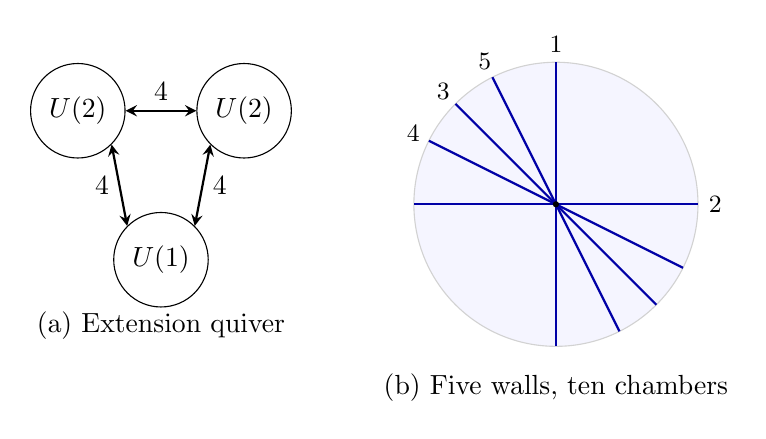
\begin{tikzpicture}[scale=.88,>=stealth]
 \node[circle,draw,minimum size=12mm] (v1) at (-4.7,1.6) {$U(2)$};
 \node[circle,draw,minimum size=12mm] (v2) at (-2.3,1.6) {$U(2)$};
 \node[circle,draw,minimum size=12mm] (v3) at (-3.5,-.55) {$U(1)$};
 \draw[<->,thick] (v1.east)--node[above]{$4$}(v2.west);
 \draw[<->,thick] (v1.south east)--node[left]{$4$}(v3.north west);
 \draw[<->,thick] (v2.south west)--node[right]{$4$}(v3.north east);
 \node at (-3.5,-1.5) {(a) Extension quiver};
 \begin{scope}[xshift=2.2cm,yshift=.25cm]
  \fill[blue!4] (0,0) circle[radius=2.05];
  \draw[gray!35] (0,0) circle[radius=2.05];
  \foreach \ang in {0,90,116.565051,135,153.434949}
    \draw[blue!65!black,thick] (\ang:2.05)--(\ang+180:2.05);
  \fill (0,0) circle[radius=.045];
  \node[font=\small] at (90:2.3) {$1$};
  \node[font=\small] at (0:2.3) {$2$};
  \node[font=\small] at (135:2.3) {$3$};
  \node[font=\small] at (153.434949:2.3) {$4$};
  \node[font=\small] at (116.565051:2.3) {$5$};
  \node at (0,-2.65) {(b) Five walls, ten chambers};
 \end{scope}
\end{tikzpicture}
\end{adjustbox}
\caption{The rank-five example. Each edge in (a) denotes four arrows in
each direction; the diagonal circle acts trivially. In (b) the horizontal
and vertical coordinates are $\zeta_1,\zeta_2$. Wall numbers refer to
Table~\ref{tab:walls}; the bounding circle has no geometric significance.}
\label{fig:quiver-walls}
\end{figure}



For each row take the simple zero-level representations for $d,e$
and scale them into the original bundle chart.
Equivariance preserves their block decomposition.
Theorem~\ref{thm:harmonic-comparison} and the local morphism
identification produce locally free $H$-stable bundles $F_d,F_e$:
their solutions are polystable, and scalar endomorphisms imply
stability. They have
\[
 v_d=\sum_i d_iv(L_i),\qquad v_e=\sum_i e_iv(L_i),\qquad
 \chi(F_d)=\chi(F_e)=0.
\]
Their $H$-slopes vanish, so their reduced $H$-Hilbert polynomials
are equal. Their distinct Mukai vectors make them nonisomorphic.

Along the corresponding line $d\cdot\zeta=0$ their slopes remain
equal. The fixed simple-orbit corrections above balance each
factor at all sufficiently small levels on this line, in the
same holomorphic isomorphism classes. Hence these factors are
stable there and their sum is polystable.
This verifies both the $H$ and the recentered real-class hypotheses
of Theorem~\ref{thm:harmonic-comparison} at every selected point.
We do not assert that all factors at every nearby wall point
are $H$-stable.

For dimension vectors $d,e$ the Mukai pairing is
\begin{equation}\label{eq:triangle-pairing}
 (v_d,v_e)=-2\sum_i d_ie_i
       +4\sum_{i<j}(d_ie_j+d_je_i).
\end{equation}
At these distinct equal-slope stable bundles, Hom in either
direction vanishes; Serre duality and Riemann--Roch identify
\eqref{eq:triangle-pairing} with the cross-extension dimension $k$.
Their self-extension dimensions are $v_d^2+2,v_e^2+2$.
This gives Table~\ref{tab:walls}, with
$\dim U=50-2k$ and transverse dimension $2(k-1)$, summing to $48$.

\subsection{Transverse contractions and metric profiles}
At a fixed selected wall point, the full local representation is
\[
 U\oplus\CC^k\oplus(\CC^k)^*,
\]
with an effective circle trivial on $U$ and of opposite weights
on the two remaining factors. Write them as $(A,B)$.
The equations and complex action are
\[
 BA=0,\qquad \|A\|^2-\|B\|^2=\kappa,\qquad
 z\cdot(A,B)=(zA,z^{-1}B).
\]
At $\kappa>0$, $A\ne0$ determines a line, and $BA=0$ identifies
the quotient with $T^*\PP^{k-1}$.
The negative sign gives the dual projective description.
At zero the invariant $N=AB$ satisfies
$N^2=0$, $\rank N\le1$, and gives the corresponding affine cone.
The two incidence maps are projective, isomorphisms over
$N\ne0$, with zero fiber $\PP^{k-1}$.

These finite contractions transport to actual local analytic
contractions on saturated neighborhoods. The full central analytic
germ is supplied by Theorem~\ref{thm:harmonic-comparison}; the
generic source charts are smooth and holomorphically identified.
For a fixed small $\kappa$, the compact exceptional fiber scales
into radius $R/2$ of a common chart. Properness of the finite
contraction makes the image of its closed complement $\{r\ge R\}$
closed and disjoint from the target origin.
Remove this image and shrink inside the central target chart.
The resulting neighborhood $U_\kappa$ has its entire inverse image
in the source chart. The contraction is therefore defined on a
full saturated neighborhood and remains proper and projective
after analytic transport. Its target neighborhood may depend on
$\kappa$; no uniform saturated radius is required.

\begin{theorem}\label{thm:k3-application}
The rank-five K3 family constructed above has the following
properties for its actual harmonic $L^2$ metric.
\begin{enumerate}
\item Near the three-factor point its full local moduli metrics
have relative error $O(|t|+|u|+r)$ from the doubled-triangle
quotients, uniformly through all stabilizer changes.
Every convergent rescaled parameter direction gives the complete
quotient limit of Theorem~\ref{thm:actual-limits}, including the
five singular wall directions and their intersection.
The finite iterated moving-center limits of
Corollary~\ref{cor:iterated-limits} apply.
\item Each wall in \eqref{eq:five-walls} has selected actual
two-factor strata with the dimensions in Table~\ref{tab:walls}.
Fix such a point and let $\kappa\to0$ with constant sign $\epsilon$.
For any sequence of base points whose balanced representatives divided
by $\sqrt{|\kappa|}$ converge to $(v_*,[A_*,B_*])$, the actual
distances divided by $\sqrt{|\kappa|}$ converge in the pointed
Gromov--Hausdorff sense to the complete product
$U\times T^*\PP^{k-1}$, based at that limit. The transverse factor
carries its flat quotient metric at level $\epsilon\in\{1,-1\}$;
for negative level the projective space has the dual description.
The actual projective exceptional fiber
has the precise $\sqrt{|\kappa|}$ diameter profile
\eqref{eq:fixed-core-scale}.
\item At zero transverse parameter, let $s$ be the nonzero singular
value of $N=AB$ and let $\mathcal S$ denote the local two-factor
stratum. In its recentered coordinates,
\[
 d^{L^2}(f_0(v,N),\mathcal S)
   =(1+O(r))\sqrt{2s}.
\]
At $N=0$ both sides vanish.
\item On the free surrounding zero-level locus,
Proposition~\ref{prop:outer-matching} gives relative matching
error $O(|t|+|u|+r+\|\zeta\|/\lambda)$ whenever
$\|\zeta\|/\lambda\to0$.
\end{enumerate}
\end{theorem}
\begin{proof}
All geometric hypotheses of Theorem~\ref{thm:harmonic-comparison}
and the existence of a module-simple point in the complex zero fiber
are verified above.
Apply Theorems~\ref{thm:actual-limits} and
\ref{thm:moving-centers} for the first assertion.
At a fixed selected wall point, the exact product normal
description and $\sqrt{|\kappa|}$ homogeneity give the second
assertion, including coverage of the whole complete product.
The saturated-domain construction identifies its compact
projective core with the actual contracted fiber.

At zero transverse level, balance gives $\|A\|=\|B\|$.
The unique nonzero singular value of $AB$ is
$s=\|A\|\|B\|$, so transverse distance to the cone vertex is
$\sqrt{\|A\|^2+\|B\|^2}=\sqrt{2s}$.
The Euclidean $U$ factor can be held fixed and cannot reduce
this transverse distance. The two-factor stratum corresponds
exactly to $U\times\{0\}$: its nearby summands stay stable and
nonisomorphic and equivariance preserves their decomposition.
Proposition~\ref{prop:stratum-distance} gives the third assertion,
even when the transverse distance is much smaller than $r$.
The fourth is the previously proved outer matching theorem.
\end{proof}

A vertex-scalar unitary negating every arrow of a triangle would
have scalar ratios $-1$ on each edge, whose product would give
$1=-1$. Thus the sufficient parity hypothesis does not apply here.
We claim the proved linear spatial error, without ruling out
additional cancellations under other normalizations.

The explicit matrices, lattice embedding and pairing formulas
above make the finite data reproducible. An accompanying exact
rational calculation checks all eleven simple representations,
their real and complex moment equations, centralizer dimensions,
and the five wall normals.\footnote{The source and exact calculation
accompany the paper in the
\href{https://github.com/bwuebben/stability-degeneration/tree/main/papers/14_quiver_metric_wall_crossing}{public repository}.}
The analytic conclusions use the
proofs above, not numerical asymptotics. All contractions and
metric limits in this application are local bundle-moduli
statements; no global Gieseker wall-crossing identification or
bubbling compactification is inferred.


\begin{thebibliography}{Wue26d}
\bibitem[AS18]{AS18}
E.~Arbarello and G.~Sacc\`a,
\textit{Singularities of moduli spaces of sheaves on K3 surfaces and
Nakajima quiver varieties}, Adv. Math. \textbf{329} (2018), 649--703.
\href{https://doi.org/10.1016/j.aim.2018.02.003}{doi:10.1016/j.aim.2018.02.003}.

\bibitem[AS25]{AS25}
E.~Arbarello and G.~Sacc\`a,
\textit{Singularities of Bridgeland moduli spaces for K3 categories: an update},
in \textit{Perspectives on Four Decades of Algebraic Geometry, Volume 1},
Progr. Math., vol.~351, Birkh\"auser, Cham, 2025, 1--42.
\href{https://doi.org/10.1007/978-3-031-66230-0_1}{doi:10.1007/978-3-031-66230-0\_1}.
Locators refer to \href{https://arxiv.org/abs/2307.07789v1}{arXiv:2307.07789v1}.

\bibitem[BeSc21]{BeSc24}
G.~Bellamy and T.~Schedler, \textit{Symplectic resolutions of quiver
varieties}, Selecta Math. (N.S.) \textbf{27} (2021), Paper No.~36.
\href{https://doi.org/10.1007/s00029-021-00647-0}{doi:10.1007/s00029-021-00647-0};
corrected text, \href{https://arxiv.org/abs/1602.00164v6}{arXiv:1602.00164v6},
July 17, 2024.

\bibitem[BS21]{BS21}
N.~Buchdahl and G.~Schumacher,
\textit{An analytic application of geometric invariant theory},
J. Geom. Phys. \textbf{165} (2021), 104237.
\href{https://doi.org/10.1016/j.geomphys.2021.104237}{doi:10.1016/j.geomphys.2021.104237};
\href{https://arxiv.org/abs/2008.04625v3}{arXiv:2008.04625v3}.

\bibitem[BS23]{BS23}
N.~Buchdahl and G.~Schumacher,
\textit{Weil--Petersson forms for families of polystable bundles over
compact K\"ahler manifolds},
Internat. J. Math. \textbf{34} (2023), no.~13, 2350082.
\href{https://doi.org/10.1142/S0129167X23500829}{doi:10.1142/S0129167X23500829}.

\bibitem[BS26]{BS26}
N.~Buchdahl and G.~Schumacher,
\textit{An explicit calculation of Weil--Petersson forms},
J. Geom. Phys. \textbf{225} (2026), 105828.
\href{https://doi.org/10.1016/j.geomphys.2026.105828}{doi:10.1016/j.geomphys.2026.105828}.

\bibitem[BZ19]{BZ19}
N.~Budur and Z.~Zhang, \textit{Formality conjecture for K3 surfaces},
Compos. Math. \textbf{155} (2019), 902--911.
\href{https://doi.org/10.1112/S0010437X19007206}{doi:10.1112/S0010437X19007206}.

\bibitem[CT24]{CT24}
A.~Clarke and C.~Tipler,
\textit{Semi-stability and local wall-crossing for Hermitian Yang--Mills connections},
J. Symplectic Geom. \textbf{22} (2024), no.~3, 673--694.
\href{https://doi.org/10.4310/JSG.241001220506}{doi:10.4310/JSG.241001220506}.
Locators refer to \href{https://arxiv.org/abs/2304.05245v1}{arXiv:2304.05245v1}.

\bibitem[CB01]{CB01}
W.~Crawley-Boevey, \textit{Geometry of the moment map for representations
of quivers}, Compos. Math. \textbf{126} (2001), 257--293.
\href{https://doi.org/10.1023/A:1017558904030}{doi:10.1023/A:1017558904030}.

\bibitem[Del25a]{DelCont25}
R.~Delloque,
\textit{Continuity of HYM connections with respect to metric variations},
J. London Math. Soc. (2) \textbf{112} (2025), no.~1, e70219.
\href{https://doi.org/10.1112/jlms.70219}{doi:10.1112/jlms.70219}.
Locators refer to \href{https://arxiv.org/abs/2403.16814v4}{arXiv:2403.16814v4}.

\bibitem[Del25b]{Del25}
R.~Delloque, \textit{Perturbations of Vector Bundle whose Curvature Form
solves a polynomial equation}, preprint, July 2025.
\href{https://arxiv.org/abs/2507.01534v1}{arXiv:2507.01534v1}.

\bibitem[Dol96]{Dol96}
I.~V.~Dolgachev, \textit{Mirror symmetry for lattice polarized K3 surfaces},
J. Math. Sci. \textbf{81} (1996), 2599--2630.
\href{https://doi.org/10.1007/BF02362332}{doi:10.1007/BF02362332};
\href{https://arxiv.org/abs/alg-geom/9502005v2}{arXiv:alg-geom/9502005v2}.

\bibitem[Gro61a]{Gro61a}
A.~Grothendieck, \textit{Techniques de construction en g\'eom\'etrie
analytique. VIII. Rapport sur les th\'eor\`emes de finitude de Grauert
et Remmert}, S\'eminaire Henri Cartan \textbf{13} (1960--1961), no.~2,
expos\'e~15, 1--10.
\href{https://numdam.org/item/SHC_1960-1961__13_2_A2_0/}{Numdam}.

\bibitem[Gro61b]{Gro61b}
A.~Grothendieck, \textit{Techniques de construction en g\'eom\'etrie
analytique. IX. Quelques probl\`emes de modules},
S\'eminaire Henri Cartan \textbf{13} (1960--1961), no.~2,
expos\'e~16, 1--20.
\href{https://numdam.org/item/SHC_1960-1961__13_2_A3_0/}{Numdam}.

\bibitem[Kin94]{King94}
A.~D.~King, \textit{Moduli of representations of finite dimensional
algebras}, Quart. J. Math. Oxford Ser. (2) \textbf{45} (1994), 515--530.
\href{https://doi.org/10.1093/qmath/45.4.515}{doi:10.1093/qmath/45.4.515}.

\bibitem[KP96]{KP96}
H.~Kraft and C.~Procesi, \textit{Classical Invariant Theory: A Primer},
preliminary version, July 1996.
\href{https://dmi.unibas.ch/fileadmin/user_upload/dmi/Personen/Kraft_Hanspeter/Classical_Invariant_Theory.pdf}{Author's text}.

\bibitem[KO97]{KO97}
K.~Kurdyka and P.~Orro, \textit{Distance g\'eod\'esique sur un sous-analytique},
Rev. Mat. Complut. \textbf{10} (1997), suppl., 173--182.
\href{https://doi.org/10.5209/rev_REMA.1997.v10.17357}{doi:10.5209/rev\_REMA.1997.v10.17357}.

\bibitem[Lun73]{Lun73}
D.~Luna, \textit{Slices \'etales},
Bull. Soc. Math. France M\'em. \textbf{33} (1973), 81--105.
\href{https://doi.org/10.24033/msmf.110}{doi:10.24033/msmf.110}.

\bibitem[May22]{May22}
M.~Mayrand, \textit{Stratification of singular hyperk\"ahler quotients},
Complex Manifolds \textbf{9} (2022), 261--284.
\href{https://doi.org/10.1515/coma-2021-0140}{doi:10.1515/coma-2021-0140}.

\bibitem[Mor84]{Mor84}
D.~R.~Morrison, \textit{On K3 surfaces with large Picard number},
Invent. Math. \textbf{75} (1984), 105--121.
\href{https://doi.org/10.1007/BF01403093}{doi:10.1007/BF01403093}.

\bibitem[NO26]{NO26}
Y.~Namikawa and Y.~Odaka, \textit{Canonical torus action on symplectic
singularities}, preprint, February 2026.
\href{https://arxiv.org/abs/2503.15791v4}{arXiv:2503.15791v4}.

\bibitem[Sta]{Stacks}
The Stacks Project Authors, \textit{The Stacks Project},
Lemma~37.53.6, Tag 0AY8.
\href{https://stacks.math.columbia.edu/tag/0AY8}{Connected fibers of proper morphisms}.

\bibitem[vD99]{vdD98}
L.~van den Dries, \textit{O-minimal structures and real analytic geometry},
in \textit{Current Developments in Mathematics, 1998},
International Press, Somerville, MA, 1999, 105--152.
\href{https://doi.org/10.4310/CDM.1998.v1998.n1.a4}{doi:10.4310/CDM.1998.v1998.n1.a4}.

\bibitem[Wue26a]{Wue26a}
B.~J.~Wuebben, \textit{Uniform Hermitian--Einstein spectra with repeated
stable factors}, preprint, October 29, 2026.
\href{https://doi.org/10.5281/zenodo.23780241}{doi:10.5281/zenodo.23780241}.

\bibitem[Wue26b]{Wue26b}
B.~J.~Wuebben, \textit{$L^2$ metrics on Hermitian--Yang--Mills moduli
spaces near a stability wall}, preprint, October 31, 2026.
\href{https://doi.org/10.5281/zenodo.23850992}{doi:10.5281/zenodo.23850992}.

\bibitem[Wue26c]{Wue26c}
B.~J.~Wuebben, \textit{Hermitian--Einstein metrics and moduli of three-step
extensions with repeated factors}, preprint, October 31, 2026.
\href{https://doi.org/10.5281/zenodo.23850994}{doi:10.5281/zenodo.23850994}.

\bibitem[Wue26d]{Wue26d}
B.~J.~Wuebben, \textit{Metric wall crossing in rank-three K3 bundle moduli},
preprint, November 6, 2026.
\href{https://doi.org/10.5281/zenodo.24021822}{doi:10.5281/zenodo.24021822}.

\bibitem[XZ26]{XZ26}
C.~Xu and Z.~Zhuang, with an appendix by H.~Guenancia,
\textit{Stable degeneration, non-degenerate forms, and Kaledin's conjecture},
preprint, June 22, 2026.
\href{https://arxiv.org/abs/2606.02401v2}{arXiv:2606.02401v2}.
\end{thebibliography}

\end{document}

